\subsection{PMT Laboratory Studies}

\subsubsection{Introduction}

Particles that pass through a medium with a higher velocity than the
phase velocity of light in that medium electromagnetically radiate
photons.  This is called {\v C}erenkov radiation.  The {\v C}erenkov 
photons are produced at an angle relative to the particle direction given by:

\begin{equation}
\cos\theta = \frac{1}{n\beta},
\end{equation}

\noindent
where $n$ is the index of refraction and $\beta=v/c$ is the particle 
velocity.

{\v C}erenkov detectors are usually used for particle identification.
Threshold {\v C}erenkov detectors make a yes/no decision based on whether 
the particle is above or below the threshold velocity $\beta_t=1/n$.
The more powerful use of {\v C}erenkov radiation comes from measuring the 
ring-correlated angles of emission of the {\v C}erenkov photons in a 
Ring Imaging {\v C}erenkov Counter (RICH).

The High Threshold {\v C}erenkov Counter for {\tt CLAS12} contains three 
main elements:

\begin{itemize}
\item a radiator through which the charged particle passes;
\item a mirror;
\item a photodetector.
\end {itemize} 

As  {\v C}erenkov radiation is a weak source of photons, light collection 
and photodetector efficiency must be as high as possible.

The number of photoelectrons ($N_{p.e.}$) per unit path length of a particle 
with charge $ze$ is:

\begin{equation}
\frac{dN_{p.e.}}{dx}=2\pi\alpha z^2\int{\frac {\epsilon(\lambda)}{\lambda^2}\displaystyle\left(1-\frac{1}{\beta^2n^2(\lambda)}\right)d\lambda},
\end{equation}

\noindent
where $x$ is the path length, $\epsilon(\lambda)$ is the efficiency for 
collecting the {\v C}erenkov light and transducing it into photoelectrons,
and $n(\lambda)$ is the index of refraction of the radiator, which is a 
function of photon energy or photon wavelength $\lambda$.  The typical 
energy-dependent variation of the index of refraction is modest, so we can 
write

\begin{equation}
\frac{dN_{p.e.}}{dx} = 2\pi\alpha z^2\displaystyle\left(1-\frac{1}{\beta^2n^2}\right)\int{\frac {\epsilon(\lambda)}{\lambda^2}d\lambda}.
\end{equation}

\noindent
The {\v C}erenkov detector quality factor (figure of merit) $N_0$ is defined 
as:

\begin{equation}
N_0 = 2\pi\alpha z^2\int{\frac {\epsilon(\lambda)}{\lambda^2}d\lambda},
\end{equation}

\noindent
So that

\begin{equation}
N_{p.e.}\approx L N_0 <sin^2\theta>,
\end{equation}

\noindent
where $L$ is the radiator length.

Careful designs of the {\v C}erenkov counter give values of $N_0$ for a 
PMT detection system working in the visible and near UV, that collect 
most of the {\v C}erenkov light of about 100~cm$^{-1}$.

The overall efficiency and rejection factors of the {\v C}erenkov counters 
are controlled by Poisson fluctuations, which can be especially critical for 
the separation of species where one particle type is dominant.  The 
effective number of photoelectrons is often less than the average number 
calculated above due to additional noise from the photodetector.  So, it is 
extremely important to design the detector with as high an average number of 
photoelectrons as possible.

The number of detected photoelectrons ($N_{p.e.}$), which is directly 
connected with the efficiency for collecting the {\v C}erenkov light and 
transducing it in photoelectrons $\epsilon(\lambda)$, contains several 
components:

\begin{equation}
\epsilon(\lambda) = \epsilon_{gas}(\lambda)\times\epsilon_{mirror}(\lambda)\times\epsilon_{PMT}(\lambda),
\end{equation}

\noindent
where $\epsilon_{gas}(\lambda)$ is the gas transparecy,
$\epsilon_{mirror}(\lambda)$ is the mirror reflectivity, and
$\epsilon_{PMT}(\lambda)$ is the PMT quantum efficiency.

One of the ways to increase the figure of merit $N_0$ is to use a PMT with 
a quartz input window.  The intensity of the photons produced in 
{\v C}erenkov radiation varies as $dN/d\lambda\sim1/\lambda^2$.  Therefore, 
it is critical to use PMTs that are efficient at low wavelengths where most 
of the light is produced.  The wavelength cutoff for a quartz PMT is in the 
region from 160--180~nm, in comparison with the 220--240~nm range for the 
UV glass PMT.  However, the quartz PMTs are more expensive.
 
\subsubsection{{\v C}erenkov Light Detection}
\label{sec:Cerenkov-Light-Detection}

The High Threshold {\v C}erenkov Counter (HTCC) for {\tt CLAS12} will 
contain a total of 48 mirrors and 48 PMTs.  The shape of the mirrors
and distribution of the PMTs for one sector of the detector is illustrated
in Fig.~\ref{HTCC_design}.  Two different types of PMTs were considered for 
the {\v C}erenkov Counters: the Photonis XP4508 quartz-faced PMT and the 
XP4500 UV glass-faced PMT.  Both models have uniform electron collection 
over their bialkali photocathodes and measure 5~in in diameter.  However, 
as seen in Fig.~\ref{quanteff_absorb}, the quartz PMTs are expected to have 
better quantum efficiency at low wavelengths than the UV glass PMTs. With 
increased efficiency, the quartz PMT should be able to detect more photons 
at higher energies than standard UV glass PMTs.
 
To study the performance of PMTs, a cosmic ray stand was used, which is 
described in Section~\ref{cosmicstand}.  In addition to studies of light 
collection by two different PMT types, we also measured the impact on light 
collection from different gas environments.  We used air and nitrogen.
Note that the HTCC will use CO$_2$ gas, but we will neglect the difference 
between CO$_2$ and nitrogen gas in our tests.  Nitrogen gas absorbs less 
light than air at low wavelengths.  The absorption factor of a gas, detailed 
in Fig.~\ref{quanteff_absorb}, is the fraction of light that the gas will 
allow to pass through it.  PMTs in a nitrogen gas environment should be able 
to detect more {\v C}erenkov light than those in air due to this improved 
transparency at low wavelengths. 

%%%%%%%%%%%%%%%%%%%%%%%%%%%%%%%%%%%%%%%%%%%%%%%%%%%%%%%%%%%%%%%%%%%%%%%
\begin{figure}
\hspace{0.5cm}
\begin{centering}
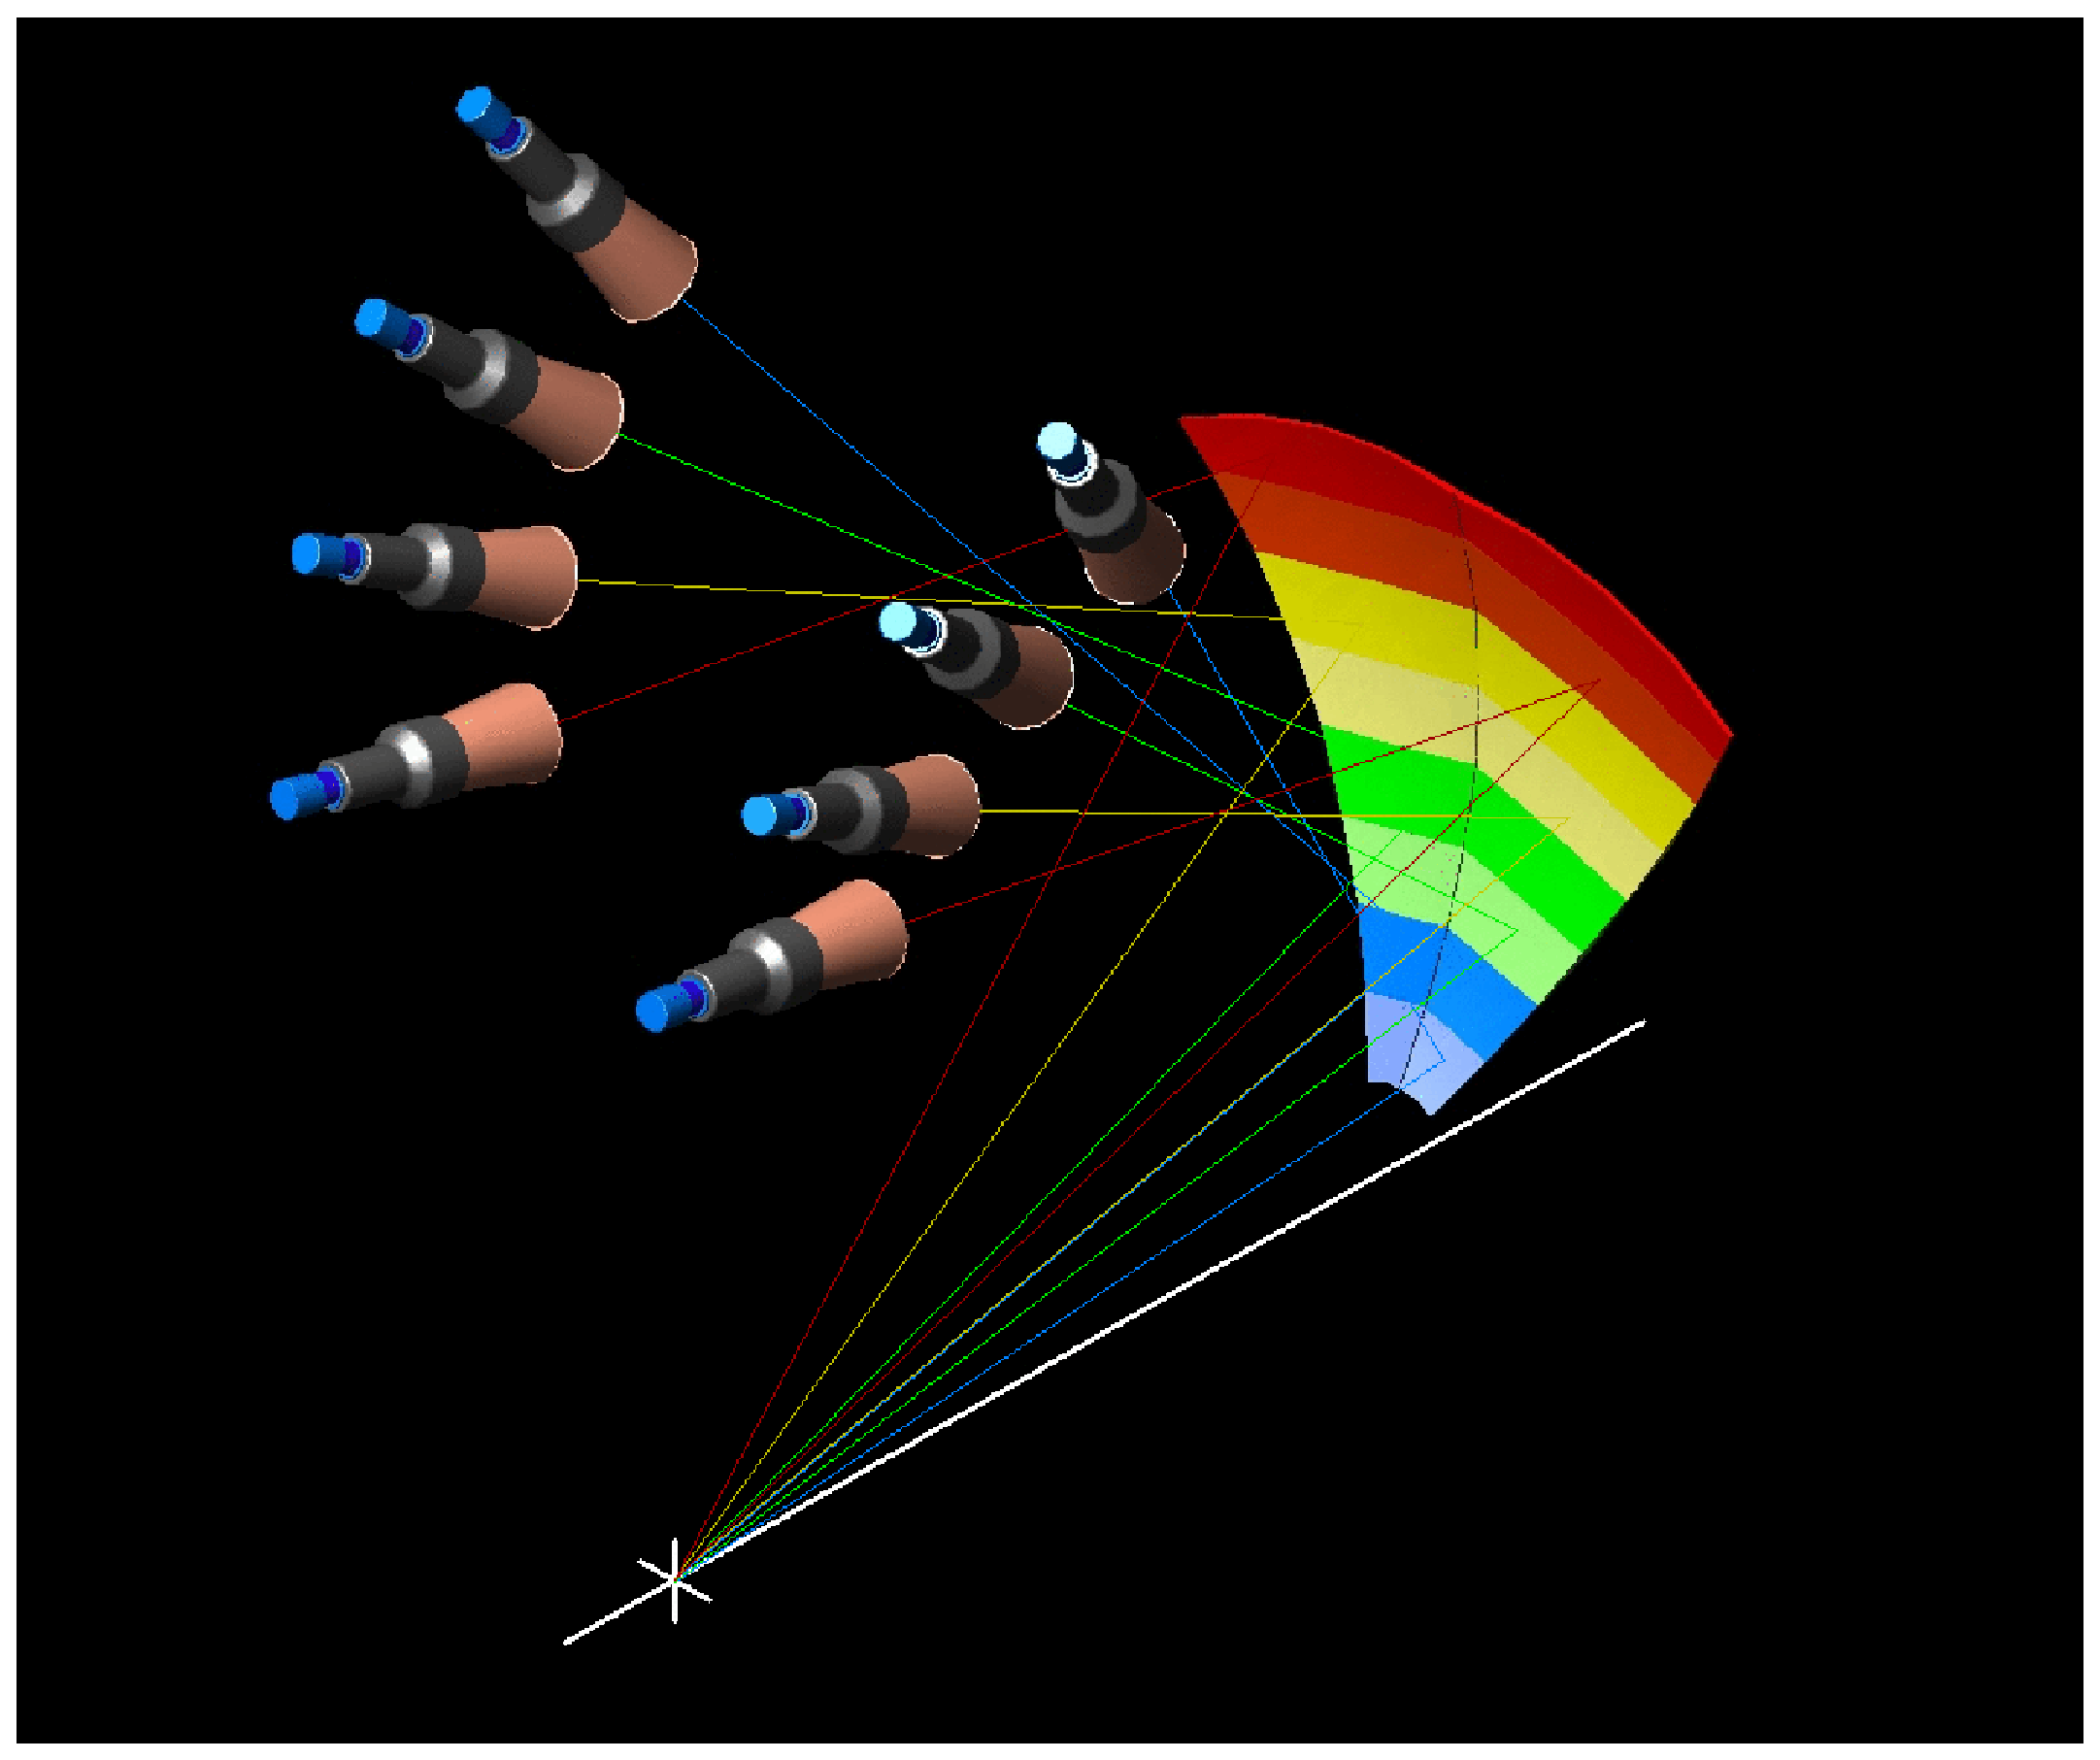
\includegraphics[height=9.0cm]{PMT-studies/vpk_2.eps}
\vspace{0.5cm}
\caption{\small{The current optical design for one sector of the HTCC. 
Eight PMTs will collect the {\v C}erenkov light reflected off of four 
mirrors.}}
\label{HTCC_design}
\end{centering}
\end{figure}
%%%%%%%%%%%%%%%%%%%%%%%%%%%%%%%%%%%%%%%%%%%%%%%%%%%%%%%%%%%%%%%%%%%%%%%

%%%%%%%%%%%%%%%%%%%%%%%%%%%%%%%%%%%%%%%%%%%%%%%%%%%%%%%%%%%%%%%%%%%%%%%
\begin{figure}
\vspace{0.5cm}
\begin{centering}
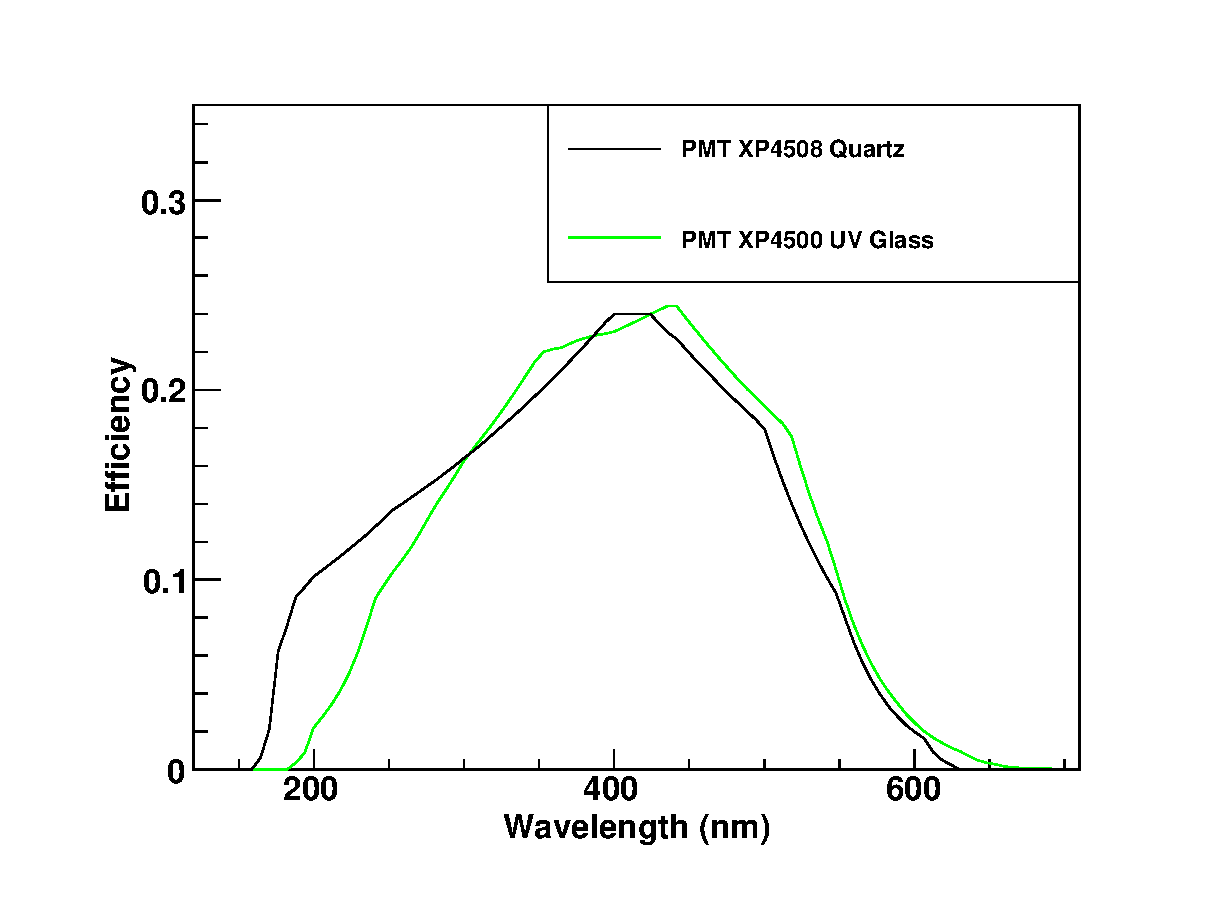
\includegraphics[height=6.0cm]{PMT-studies/pmt_2.eps}
\includegraphics[height=6.0cm]{PMT-studies/pmt_1.eps}
\vspace{0.5cm}
\caption{\small{Left: The quantum efficiency as a function of wavelength 
of the two Photonis PMT models being tested. Right: The absorption factors 
of nitrogen gas and air as a function of wavelength.}}
\label{quanteff_absorb}
\end{centering}
\end{figure}
%%%%%%%%%%%%%%%%%%%%%%%%%%%%%%%%%%%%%%%%%%%%%%%%%%%%%%%%%%%%%%%%%%%%%%%

Multiplying the gas absorption factor by the PMT quantum efficiency
and the $1/\lambda^2$ {\v C}erenkov light production dependence
gives, to a constant factor, the amount of {\v C}erenkov light collected
as a function of wavelength. The predicted amounts of light collected
for different gas and PMT-face configurations are plotted in 
Fig.~\ref{light_comparison}.  Taking the ratio of their integrals
for quartz and UV-glass in air gives:

\begin{equation}
\label{eq:light_ratio}
\frac{\textrm{Light}_{Quartz,\textrm{ }Air}}
{\textrm{Light}_{UV-Glass,\textrm{ }Air}} = 
\frac{\int_{0}^{\infty}QE_{Quartz}(\lambda)*AF_{Air}(\lambda)/\lambda^2d\lambda}
{\int_{0}^{\infty}QE_{UV-Glass}(\lambda)*AF_{Air}(\lambda)/\lambda^2\lambda}
= 1.2,
\end{equation}

\noindent
yielding a predicted 20\% improvement in light collection. Similarly,
in a nitrogen gas environment, this improvement increases to 25\%.
However, comparing the air and nitrogen gas environments for the quartz-faced
PMTs only results in a 4.5\% predicted increase in light collection.
The UV glass-faced PMT is predicted to achieve no appreciable improvement
in light collection in a nitrogen gas. This is because the quantum
efficiency of the XP4500 rapidly approaches zero for light with 
$\lambda < 200$~nm, the region where nitrogen gas has the most improvement 
over air.  These predictions are only preliminary, rough estimates as the
quantum efficiency measurements of the PMTs supplied by the manufacturer
are only characteristic approximations. 

%%%%%%%%%%%%%%%%%%%%%%%%%%%%%%%%%%%%%%%%%%%%%%%%%%%%%%%%%%%%%%%%%%%%%%%
\begin{figure}
\vspace{0.5cm}
\begin{centering}
\includegraphics[height=5.5cm]{PMT-studies/pmt_6.eps}
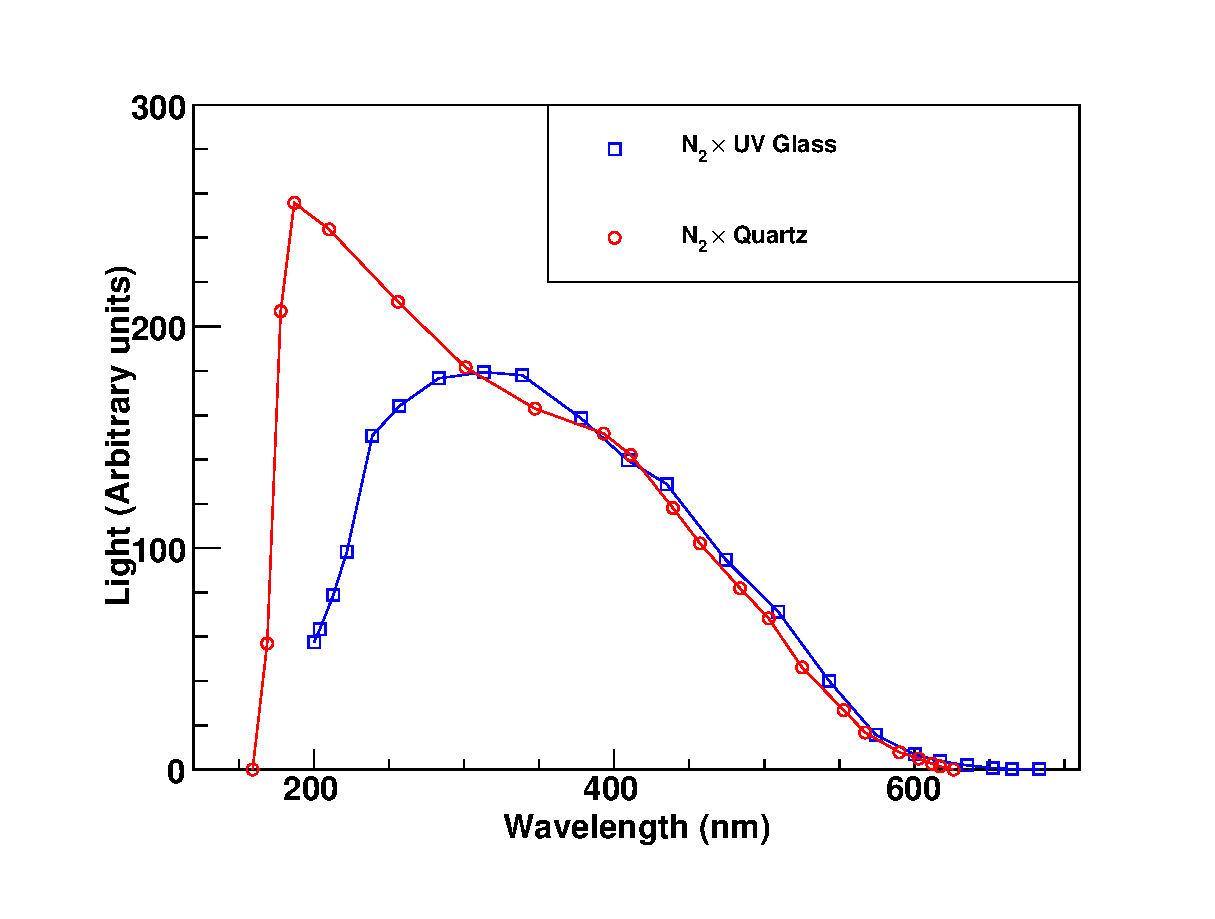
\includegraphics[height=5.5cm]{PMT-studies/pmt_5.eps}
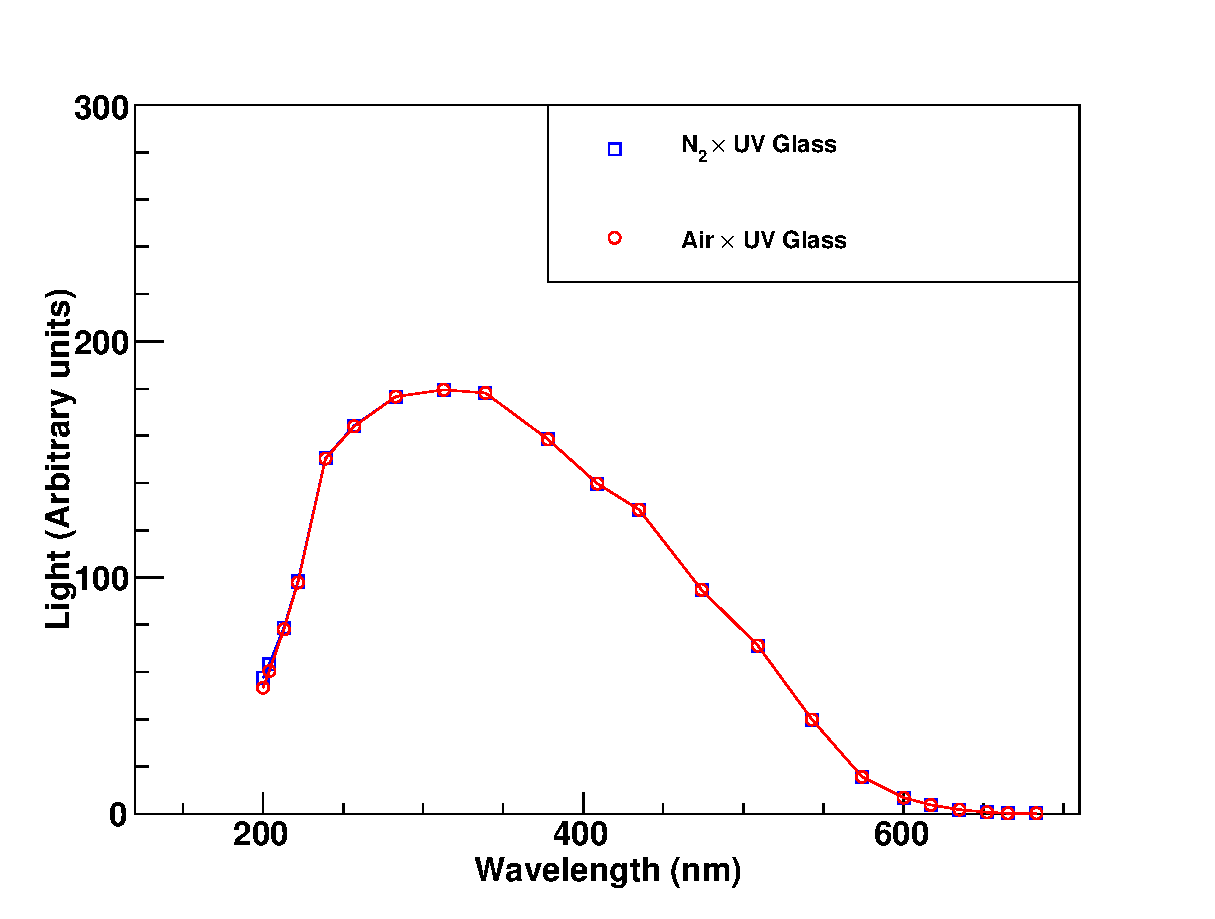
\includegraphics[height=5.5cm]{PMT-studies/pmt_3.eps}
\includegraphics[height=5.5cm]{PMT-studies/pmt_4.eps}
\vspace{0.5cm}
\caption{\small{To a constant factor, the predicted amount of light collected 
as a function of wavelength for different PMT face and gas configurations,
plotted against each other for comparison.}}
\label{light_comparison}
\end{centering}
\end{figure}
%%%%%%%%%%%%%%%%%%%%%%%%%%%%%%%%%%%%%%%%%%%%%%%%%%%%%%%%%%%%%%%%%%%%%%%

\subsubsection{Cosmic Ray Stand}
\label{cosmicstand}

The predicted increase of detected photoelectrons in quartz-faced
PMTs is significant, so a test stand (see Fig.~\ref{test_stand})
was constructed to determine whether this performance increase is
reproducible.  A stack of 32 quartz plates was used as a medium for
{\v C}erenkov light generation as cosmic muons passed through them.
As diagrammed in Fig.~\ref{test_stand}, the {\v C}erenkov light was 
produced at a 46.7$^\circ$ angle from the incoming cosmic rays and was 
internally reflected until passing out of the end of the quartz plate. In 
a light-tight and air-tight box, the {\v C}erenkov radiation emitted by 
these cosmic rays was collected by two PMTs located an average of 11~cm 
away from the quartz plates.  While one of the PMTs was being tested, a 
second PMT was used as a reference to confirm the consistency of the 
experiment from test to test.  Three Photonis XP4508 quartz-faced PMTs and 
three Photonis XP4500 UV glass-faced PMTs were tested in air, and one of 
each type in nitrogen gas, which is close in optical properties to CO$_2$, 
which will be used in the HTCC.  A flow meter and pressure gauge were used 
to regulate the supply of nitrogen gas to the chamber during the final tests. 

%%%%%%%%%%%%%%%%%%%%%%%%%%%%%%%%%%%%%%%%%%%%%%%%%%%%%%%%%%%%%%%%%%%%%%%
\begin{figure}
\vspace{0.5cm}\begin{centering}
\includegraphics[height=5.0cm]{PMT-studies/IMG_0196.eps}
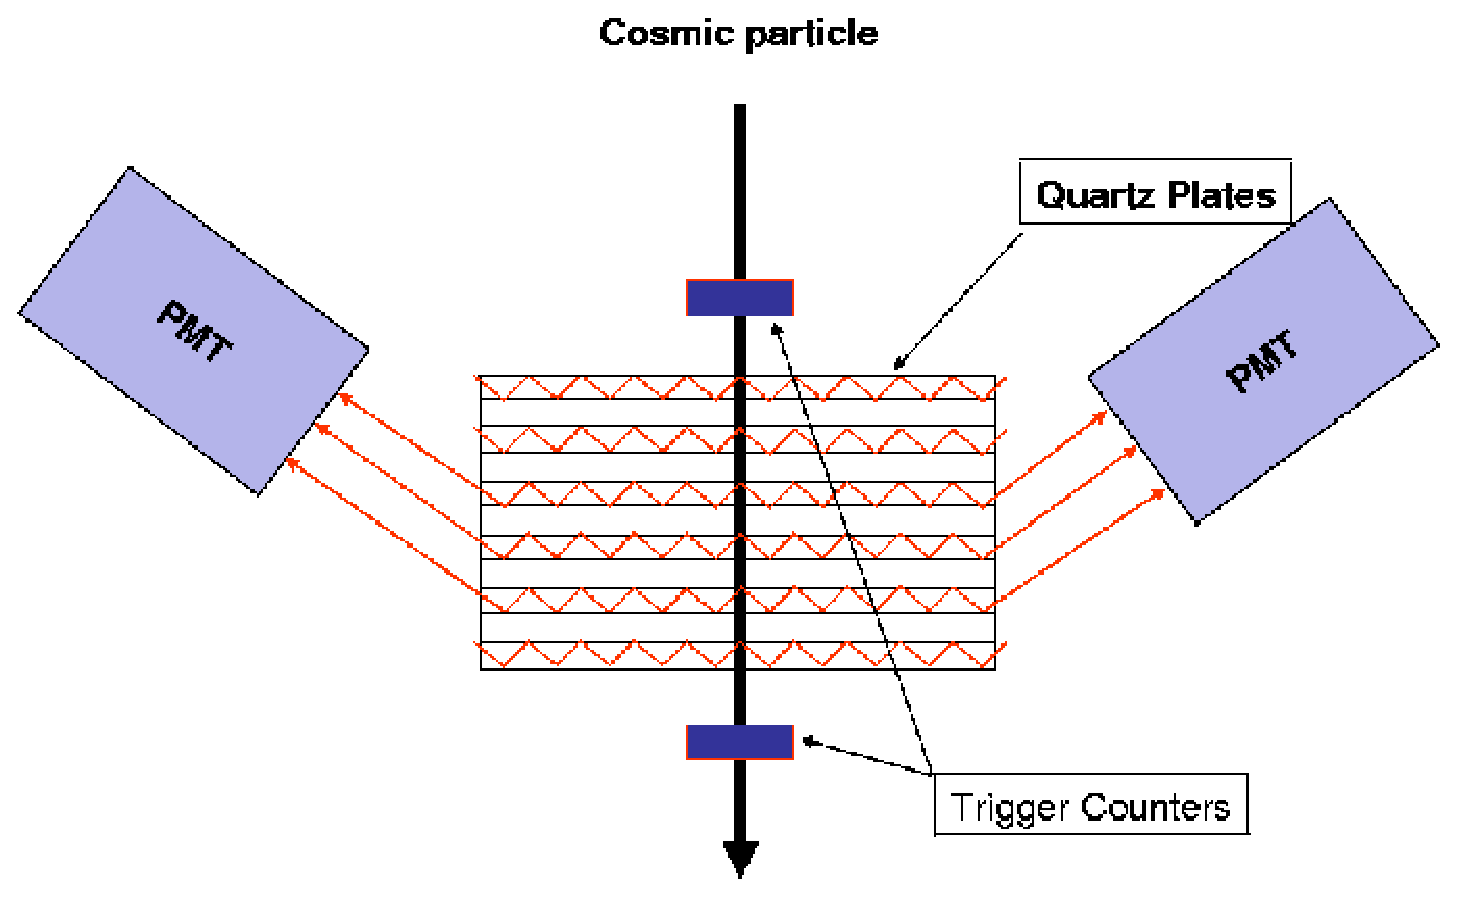
\includegraphics[height=5.0cm]{PMT-studies/cc_test.eps}
\vspace{0.5cm}
\caption{\small{A photograph (left) and schematic (right) of the cosmic 
ray stand used for testing the {\v C}erenkov light collection of different 
PMTs.  Trigger counters above and below the chamber detect a signal when 
a cosmic ray has passed through the quartz plates, and the two PMTs collect
the resulting {\v C}erenkov radiation. A flow meter and pressure gauge
are used to supply and regulate nitrogen gas to the chamber.}}
\label{test_stand}
\end{centering}
\end{figure}
%%%%%%%%%%%%%%%%%%%%%%%%%%%%%%%%%%%%%%%%%%%%%%%%%%%%%%%%%%%%%%%%%%%%%%%

To collect data, small scintillators attached to PMTs above and below
the test chamber were used to trigger event recording. A coincidence
between both PMTs indicated that a cosmic ray had passed through the
quartz plates, producing {\v C}erenkov light.  The trigger and data
acquisition systems are pictured and diagrammed in Fig.~\ref{trig_daq}.
The pulse height of the electrical signals from the PMT dynodes were
converted to digital ADCs for analysis. The ADC spectra of the two
trigger counters and the two {\v C}erenkov counters for one test run
are shown in Fig.~\ref{sample_adc}.  Cuts were placed around the peaks 
of the ADC spectra of the trigger PMTs to remove background events.  Also, 
the high voltage supplied to the PMTs was fixed throughout the experiment 
to make sure that the response of each of the PMTs was consistent. 

%%%%%%%%%%%%%%%%%%%%%%%%%%%%%%%%%%%%%%%%%%%%%%%%%%%%%%%%%%%%%%%%%%%%%%%
\begin{figure}
\vspace{0.5cm}\begin{centering}
\includegraphics[height=5.0cm]{PMT-studies/cerenk-daq.eps}
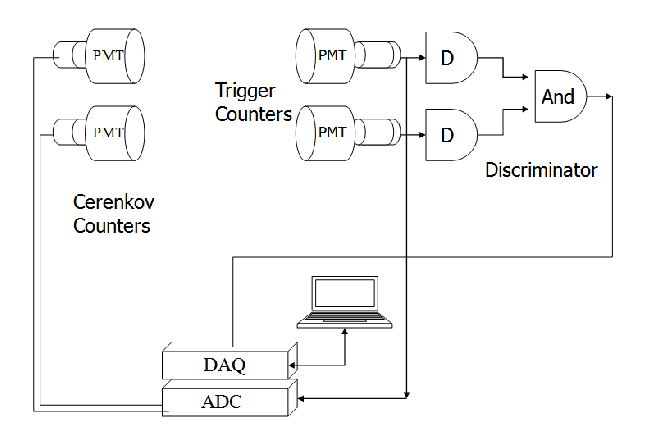
\includegraphics[height=5.0cm]{PMT-studies/daq.eps}
\vspace{0.5cm}
\caption{\small{Left: Data acquisition hardware. Right: Diagram of the 
triggering and DAQ process.}}
\label{trig_daq}
\end{centering}
\end{figure}
%%%%%%%%%%%%%%%%%%%%%%%%%%%%%%%%%%%%%%%%%%%%%%%%%%%%%%%%%%%%%%%%%%%%%%%

%%%%%%%%%%%%%%%%%%%%%%%%%%%%%%%%%%%%%%%%%%%%%%%%%%%%%%%%%%%%%%%%%%%%%%%
\begin{figure}
\vspace{0.5cm}\begin{centering}
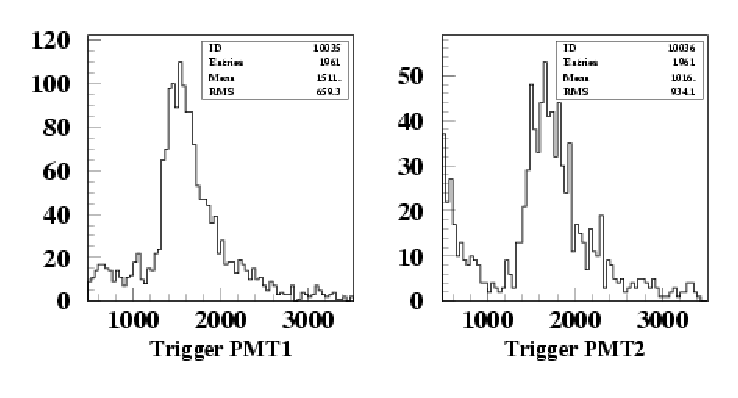
\includegraphics[height=5.0cm]{PMT-studies/triggers.eps}
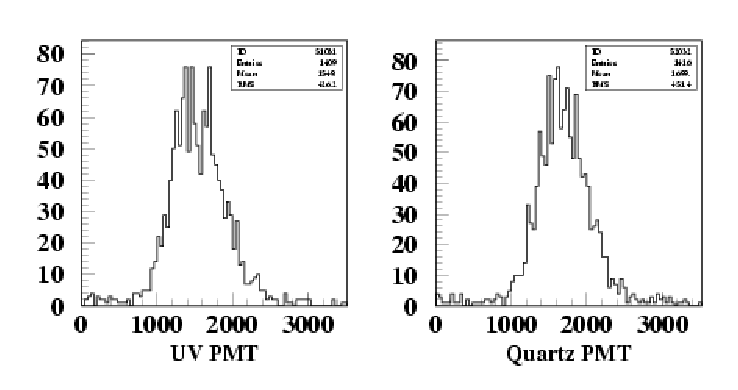
\includegraphics[height=5.0cm]{PMT-studies/cerenk_counters.eps}
\vspace{0.5cm}
\caption{\small{ADC spectra of the two trigger counters (top) and two 
{\v C}erenkov counters (bottom) for one test run.}}
\label{sample_adc}
\end{centering}
\end{figure}
%%%%%%%%%%%%%%%%%%%%%%%%%%%%%%%%%%%%%%%%%%%%%%%%%%%%%%%%%%%%%%%%%%%%%%%

\subsubsection{Calibration of the ADC Scale}

The ADC spectra of the test PMTs must be converted into units of collected
number of photoelectrons ($N_{p.e.}$) to judge PMT performance.  This 
conversion is linear because the multi-stage signal amplification process 
of the PMTs is independent of the number of photons detected.  The ADC
conversion factor for each PMT was found by using an LED to fix the
source intensity.  The LED and test PMTs were placed in a light-tight
box for testing.  Multiple tests were performed for each PMT, each
with a different intensity of LED source photons. 

The energy response of a PMT to a fixed intensity source of photons
is described by a Poisson-like distribution, 

\begin{equation}
N(ADC) = \frac{N_{0}\mu^{\frac{ADC}{\mu_1}}e^{-\mu}}{\mu_{1}
\Gamma(\frac{ADC}{\mu_1}+1)},\textrm{ }\Gamma(x)=\int_0^\infty t^{x-1}e^{-t}dt,
\end{equation}

\noindent
where $\mu$ is the average number of photoelectrons, $\mu_1$ is
the ADC to $N_{p.e.}$ conversion factor, and $N_0$ is the scaling factor.
The Poisson distribution fits to the ADC spectra of different light
intensities for the three UV-glass-faced PMTs and the three quartz-faced
PMTs are shown in Figs.~\ref{poisson_uvglass} and \ref{poisson_quartz},
respectively. To find the average conversion factor, the average ADC
vs. the average $N_{p.e.}$ were plotted in Figs.~\ref{linear_uvglass}
and \ref{linear_quartz} and fit to a linear function.  The slope
of these fits gives the ADC to $N_{p.e.}$ conversion factor for each 
test PMT. 

%%%%%%%%%%%%%%%%%%%%%%%%%%%%%%%%%%%%%%%%%%%%%%%%%%%%%%%%%%%%%%%%%%%%%%%
\begin{figure}
\vspace{0.5cm}
\begin{centering}
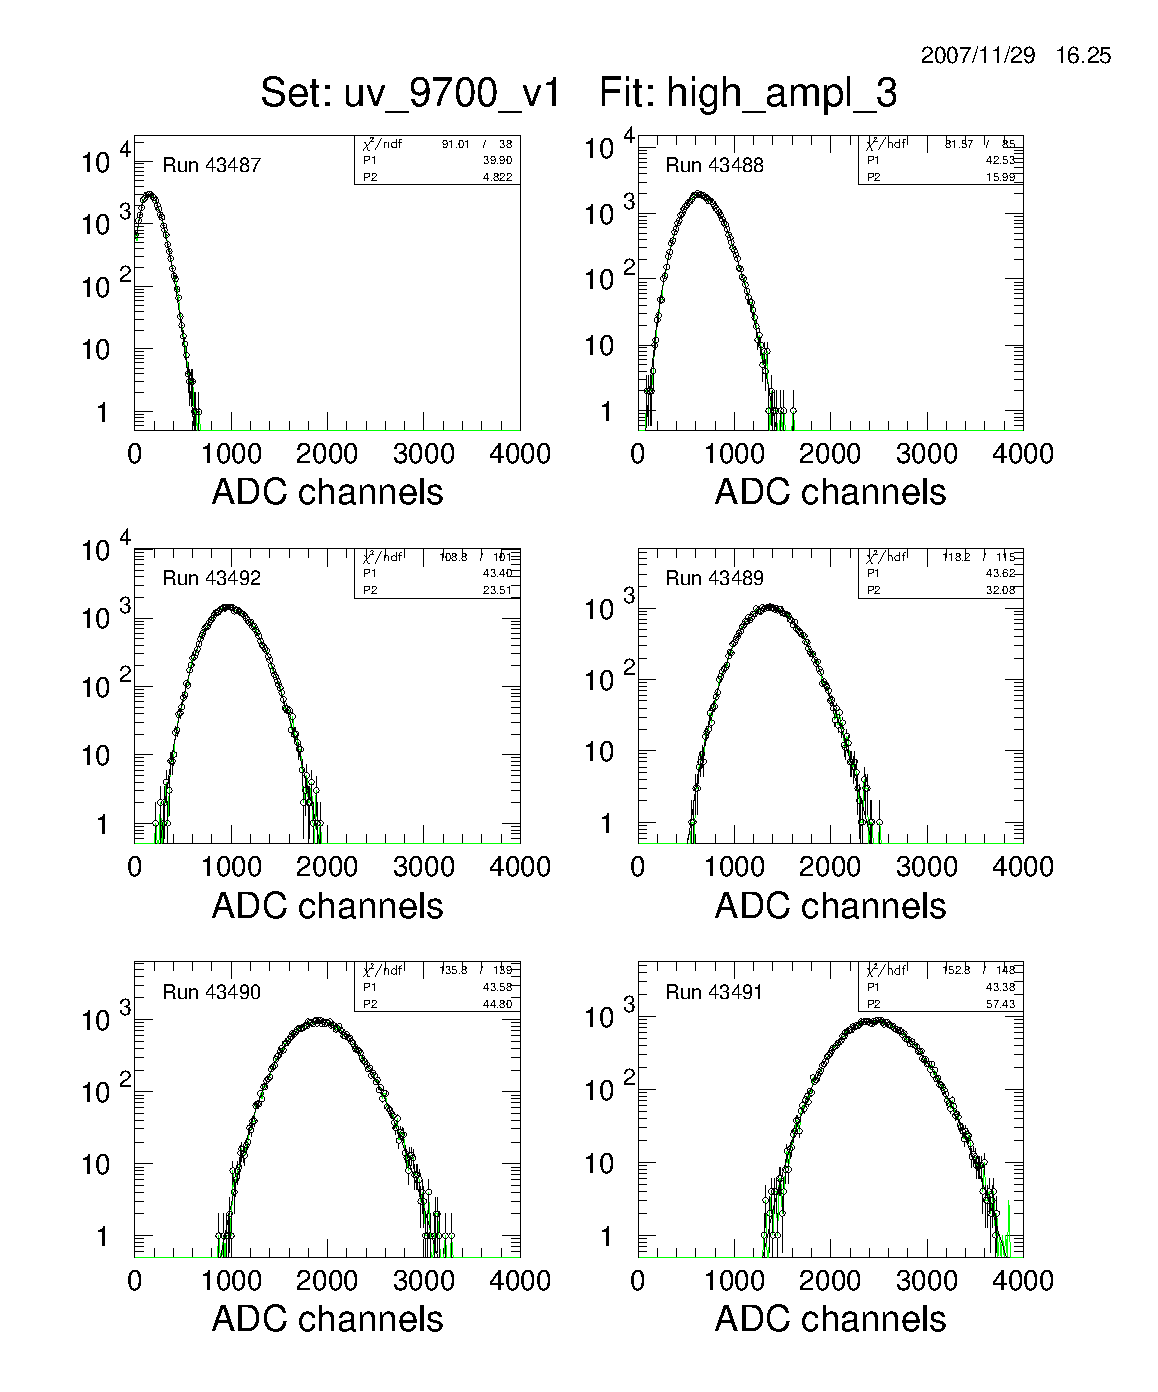
\includegraphics[height=10.0cm]{PMT-studies/uv_9700_v1_fits.eps}
\end{centering}
\begin{centering}
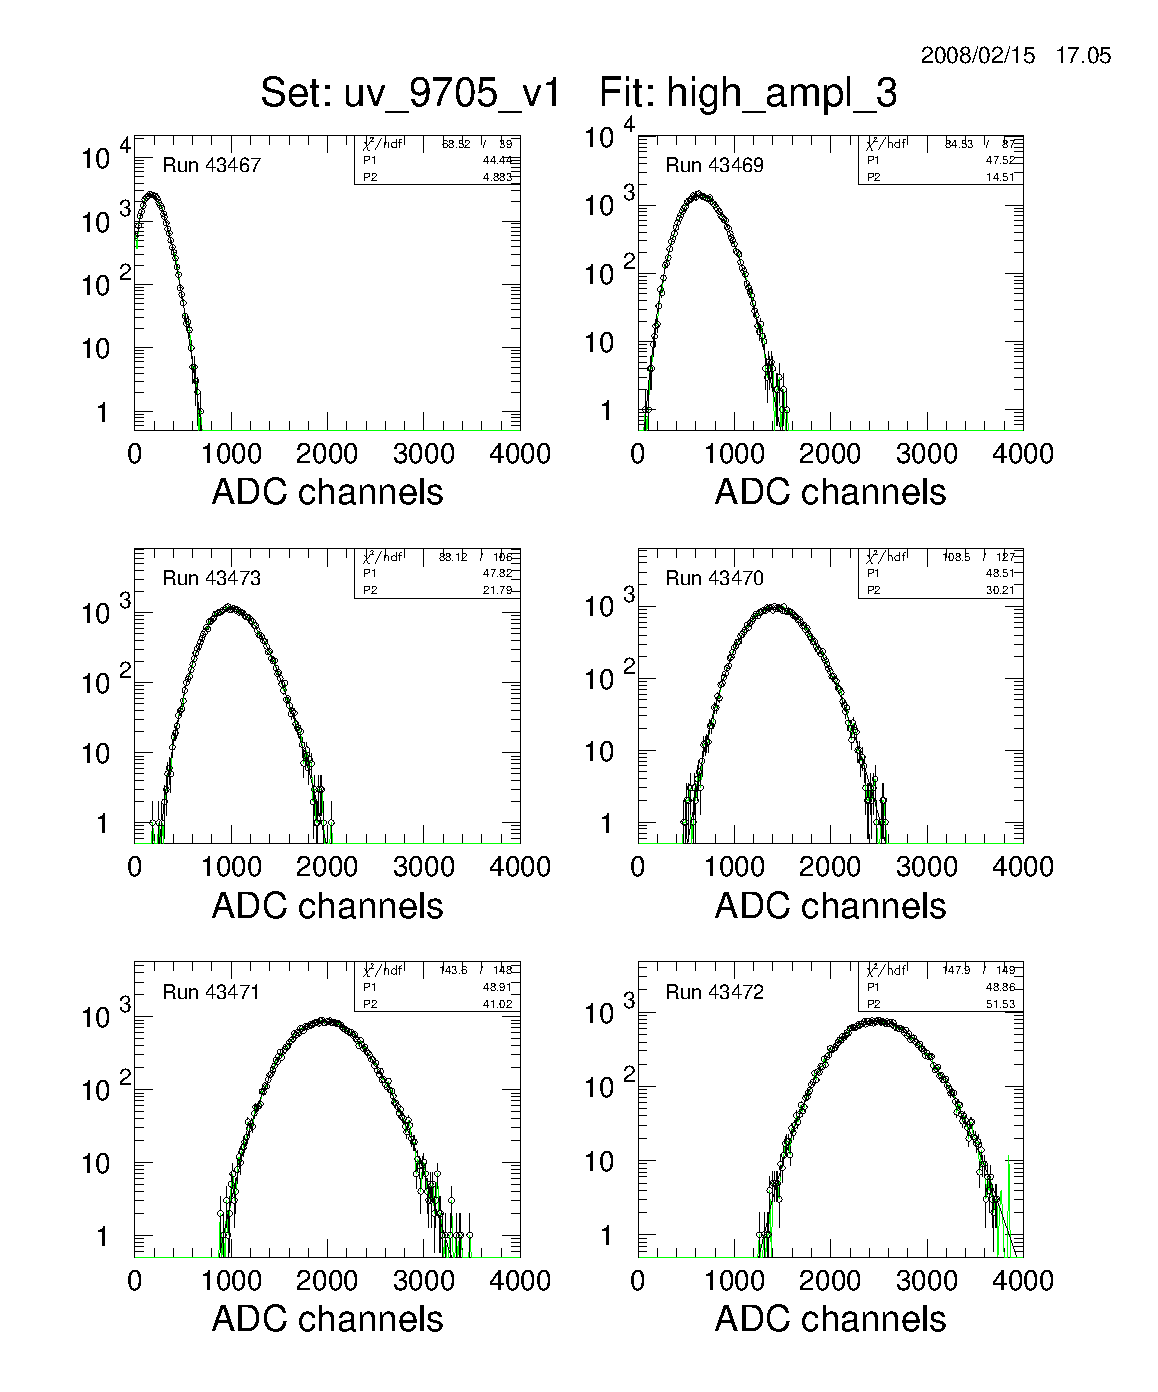
\includegraphics[height=9.5cm]{PMT-studies/uv_9705_v1_fits.eps}
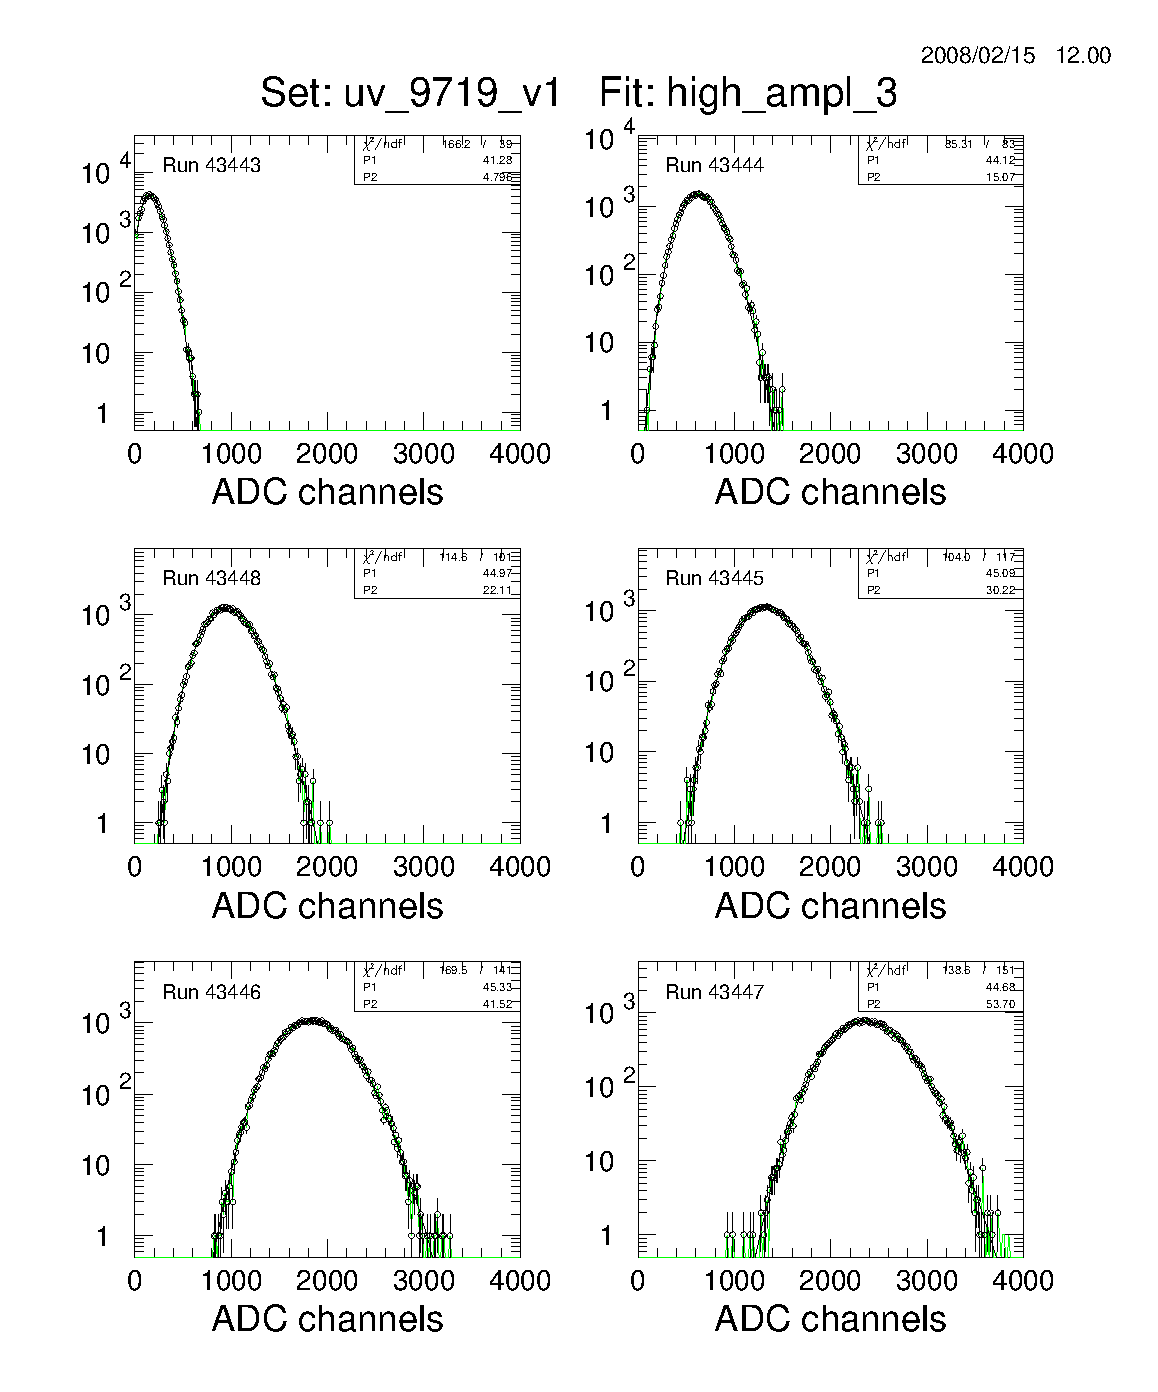
\includegraphics[height=9.5cm]{PMT-studies/uv_9719_v1_fits.eps}
\vspace{0.5cm}
\caption{\small{Poisson fits to ADC spectra of the three UV glass-faced 
PMTs.  Here, $P1$ is the ADC to $N_{p.e.}$ conversion factor $\mu_1$, and 
$P2$ is the average number of photoelectrons, $\mu$.}}
\label{poisson_uvglass}
\end{centering}
\end{figure}
%%%%%%%%%%%%%%%%%%%%%%%%%%%%%%%%%%%%%%%%%%%%%%%%%%%%%%%%%%%%%%%%%%%%%%%

%%%%%%%%%%%%%%%%%%%%%%%%%%%%%%%%%%%%%%%%%%%%%%%%%%%%%%%%%%%%%%%%%%%%%%%
\begin{figure}
\vspace{0.5cm}
\begin{centering}
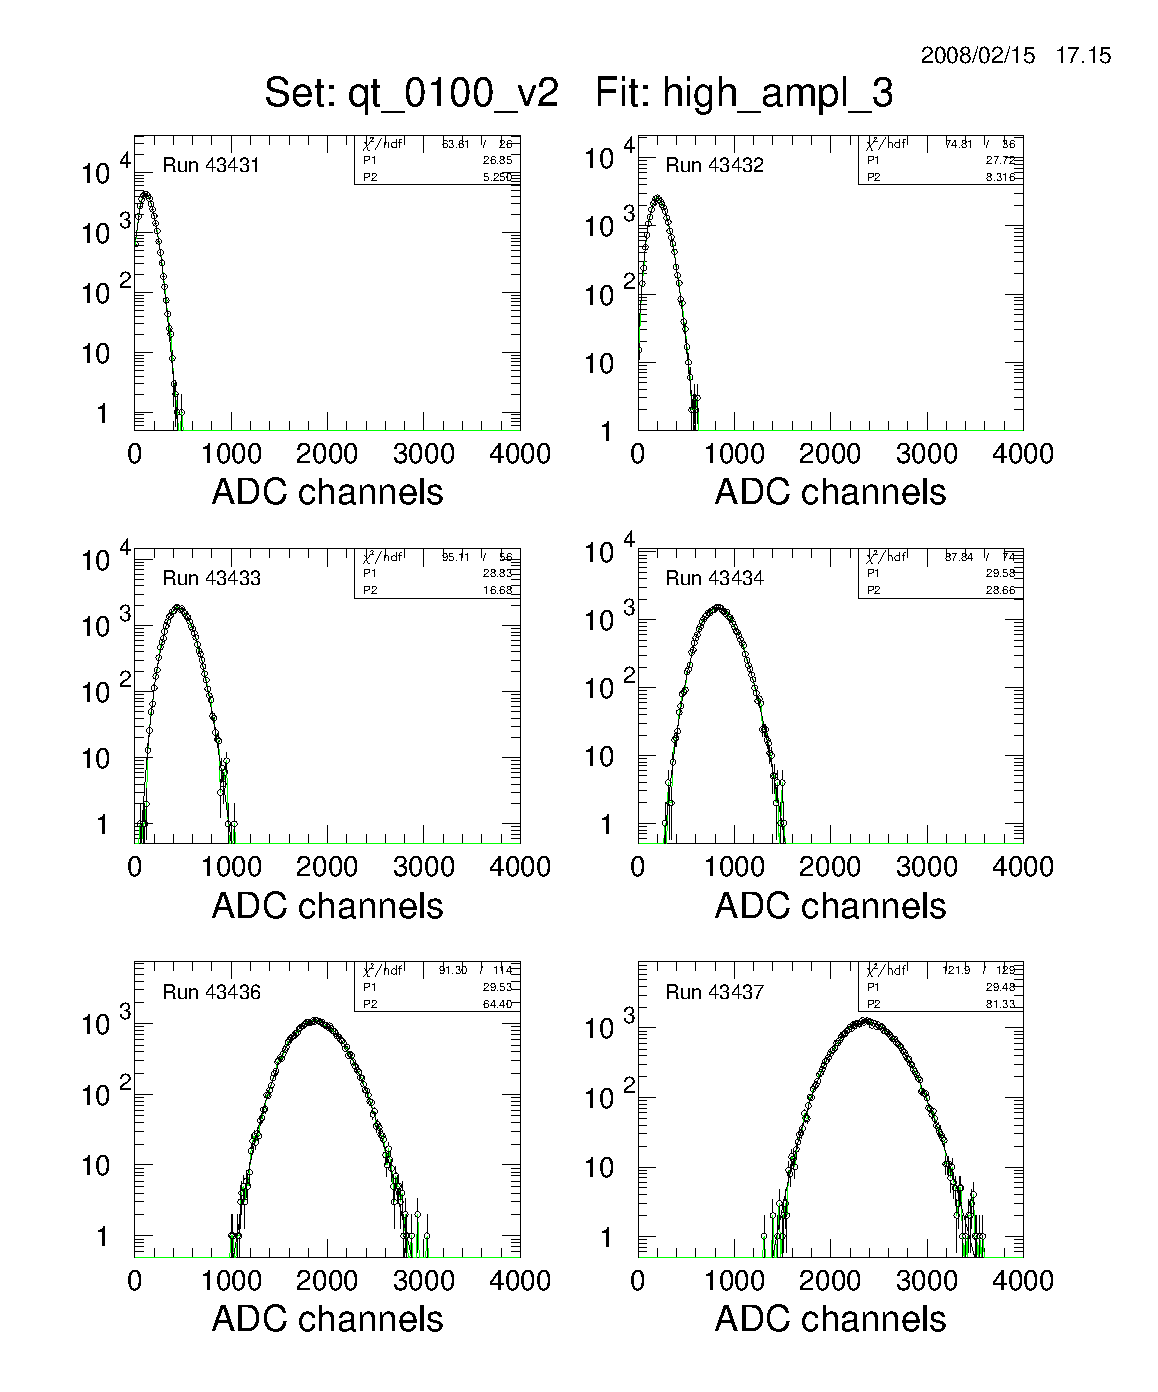
\includegraphics[height=10.0cm]{PMT-studies/qt_0100_v2_fits.eps}
\end{centering}
\begin{centering}
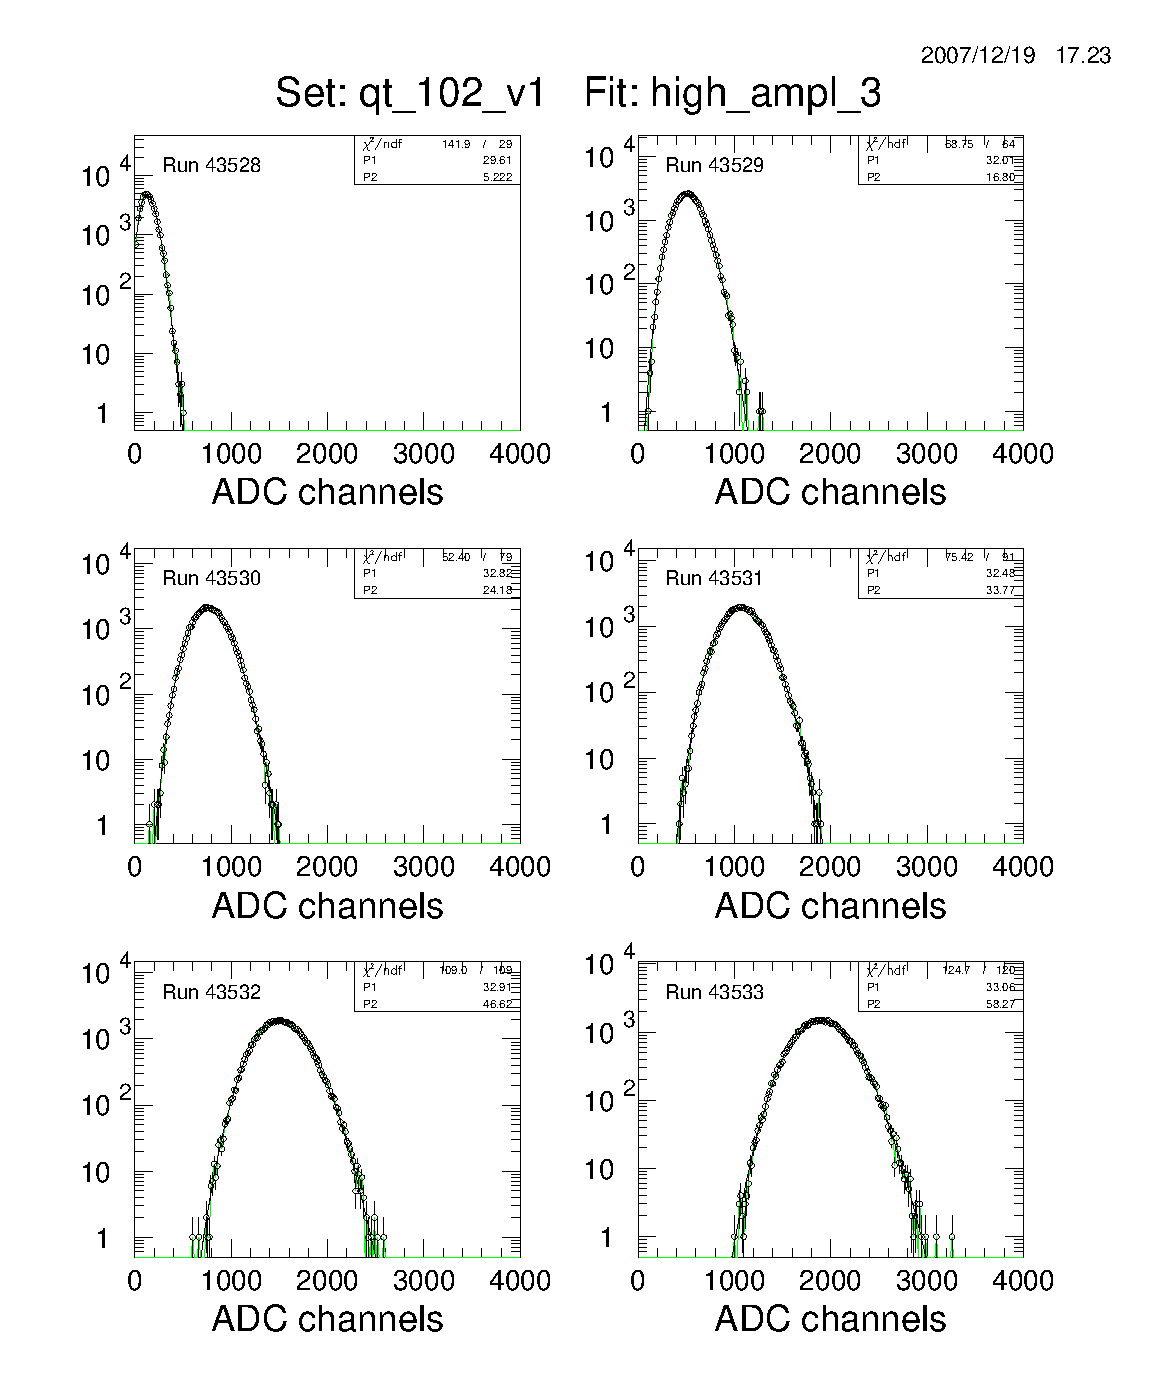
\includegraphics[height=9.5cm]{PMT-studies/qt_0102_v1_fits.eps}
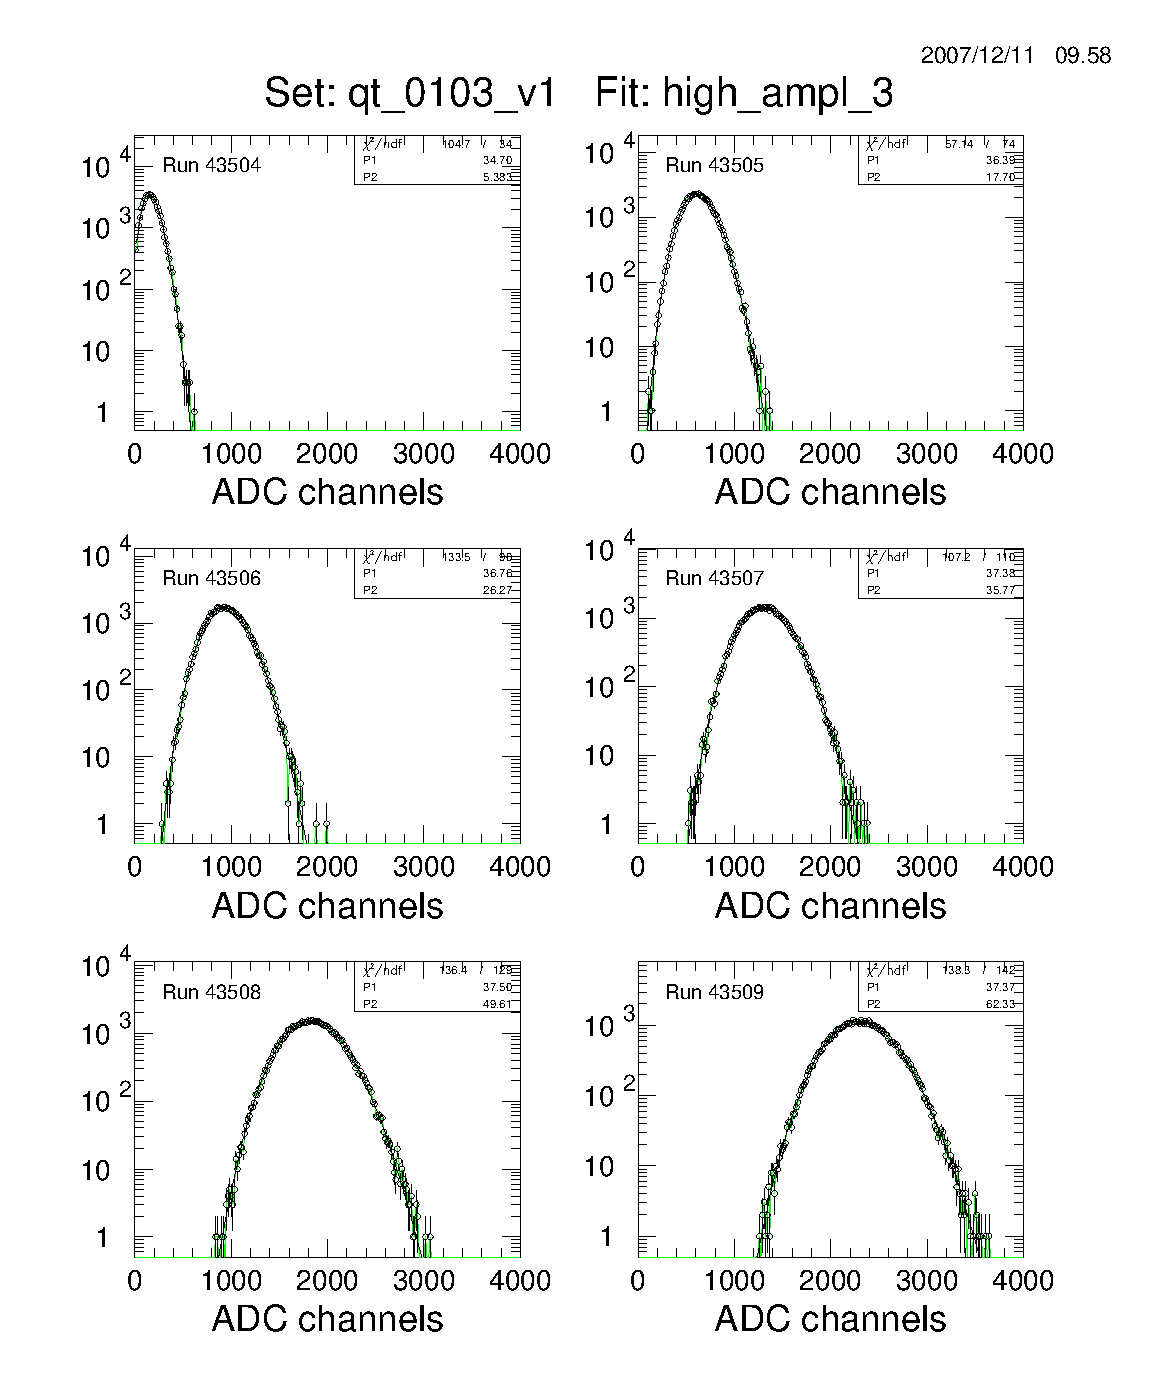
\includegraphics[height=9.5cm]{PMT-studies/qt_0103_v1_fits.eps}
\vspace{0.5cm}
\caption{\small{Poisson fits to ADC spectra of the three quartz-faced 
PMTs.  Here, $P1$ is the ADC to $N_{p.e.}$ conversion factor $\mu_1$, 
and $P2$ is the average number of photoelectrons, $\mu$.}}
\label{poisson_quartz}
\end{centering}
\end{figure}
%%%%%%%%%%%%%%%%%%%%%%%%%%%%%%%%%%%%%%%%%%%%%%%%%%%%%%%%%%%%%%%%%%%%%%%

%%%%%%%%%%%%%%%%%%%%%%%%%%%%%%%%%%%%%%%%%%%%%%%%%%%%%%%%%%%%%%%%%%%%%%%
\begin{figure}
\vspace{0.5cm}
\begin{centering}
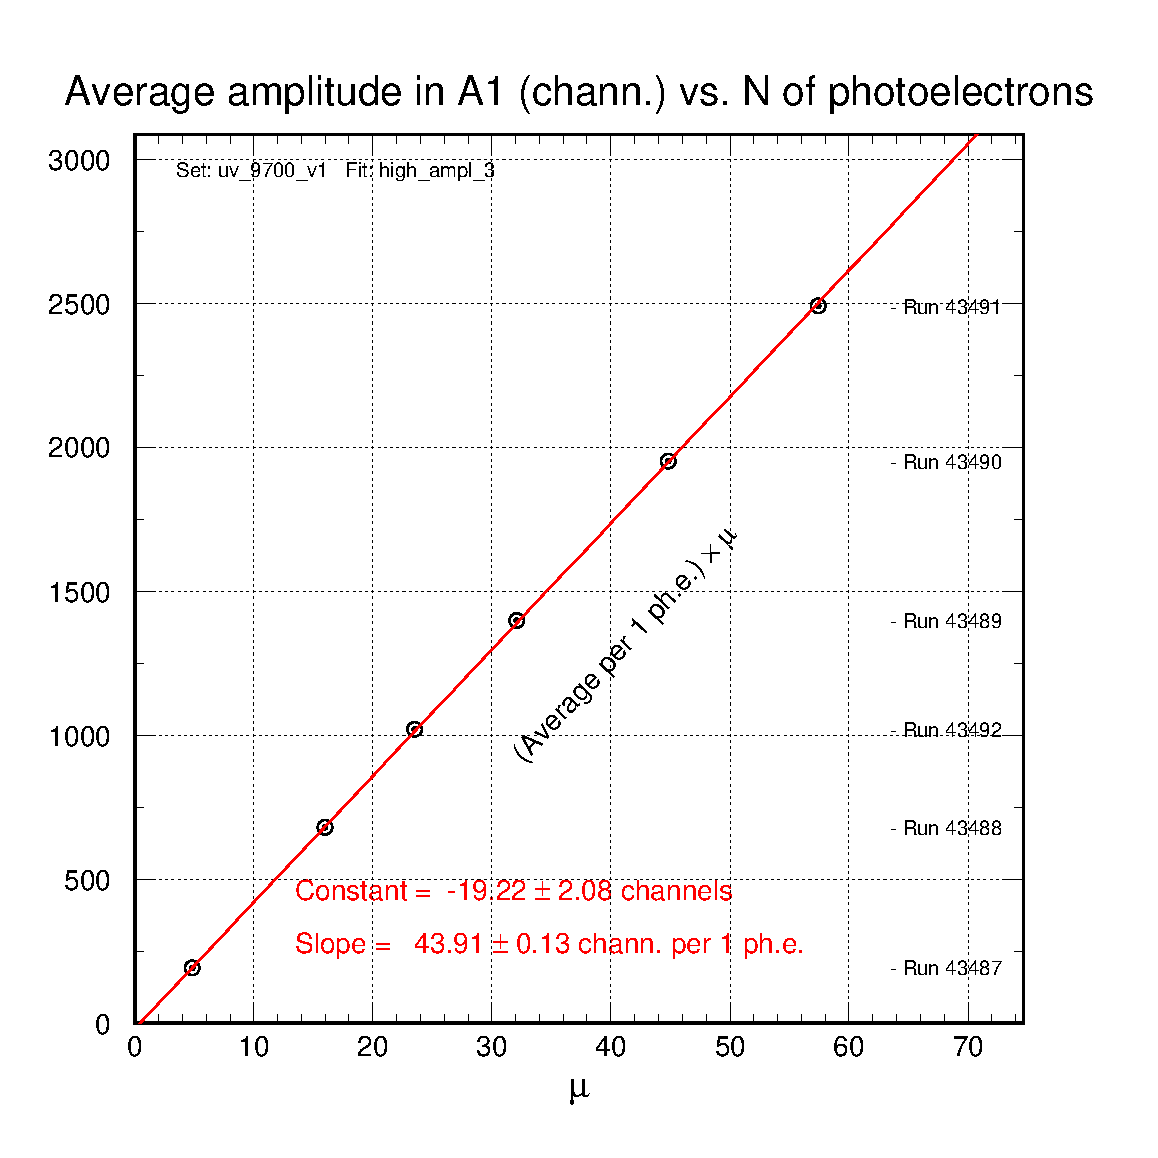
\includegraphics[height=8.5cm]{PMT-studies/uv_9700_v1_result.eps}
\end{centering}
\begin{centering}
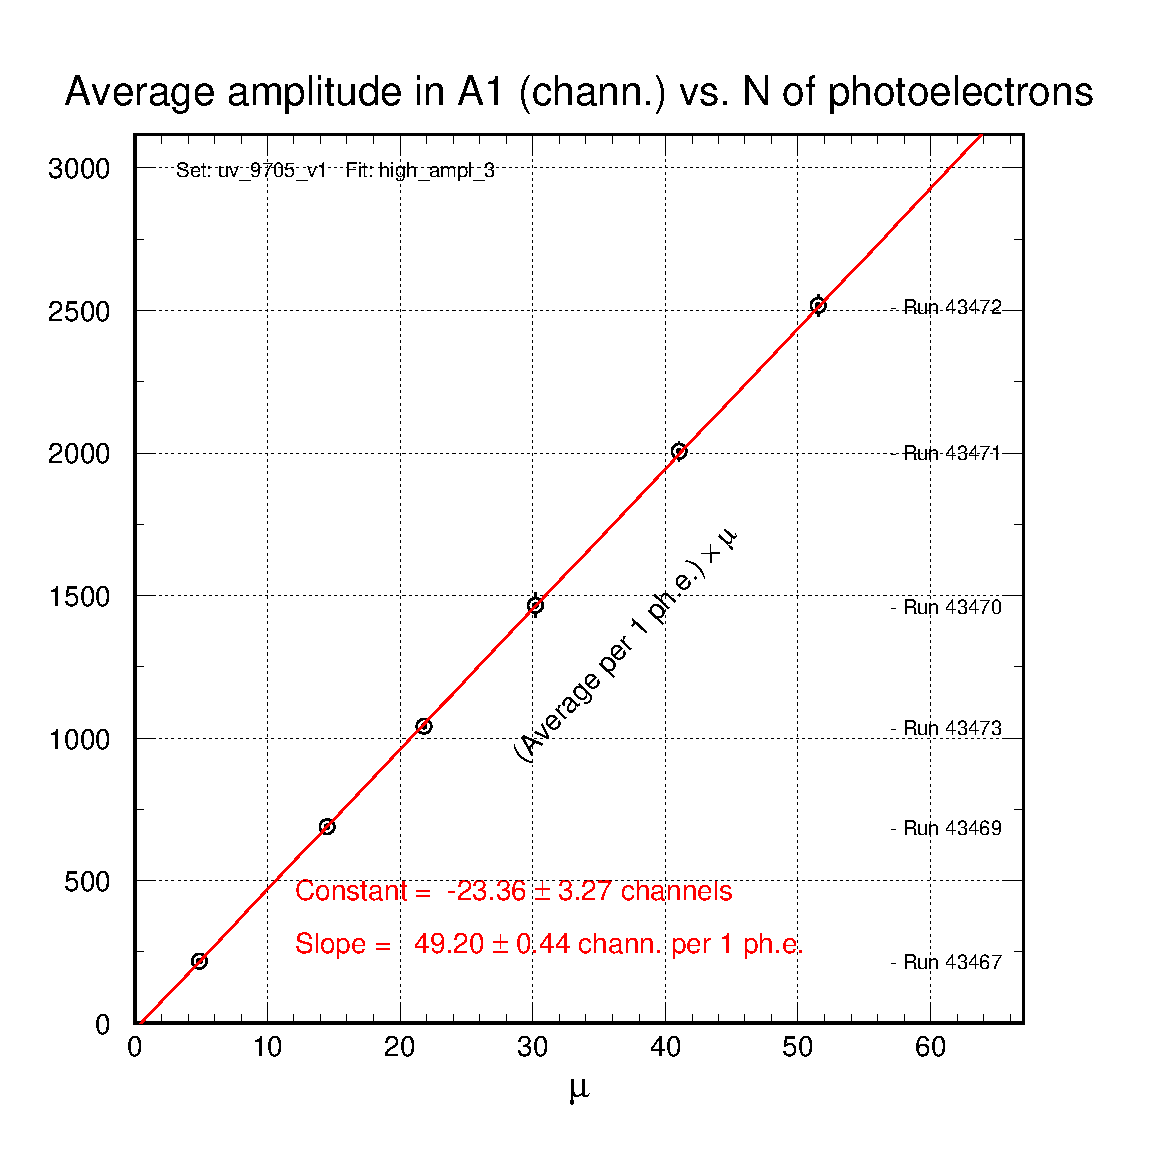
\includegraphics[height=8.0cm]{PMT-studies/uv_9705_v1_result.eps}
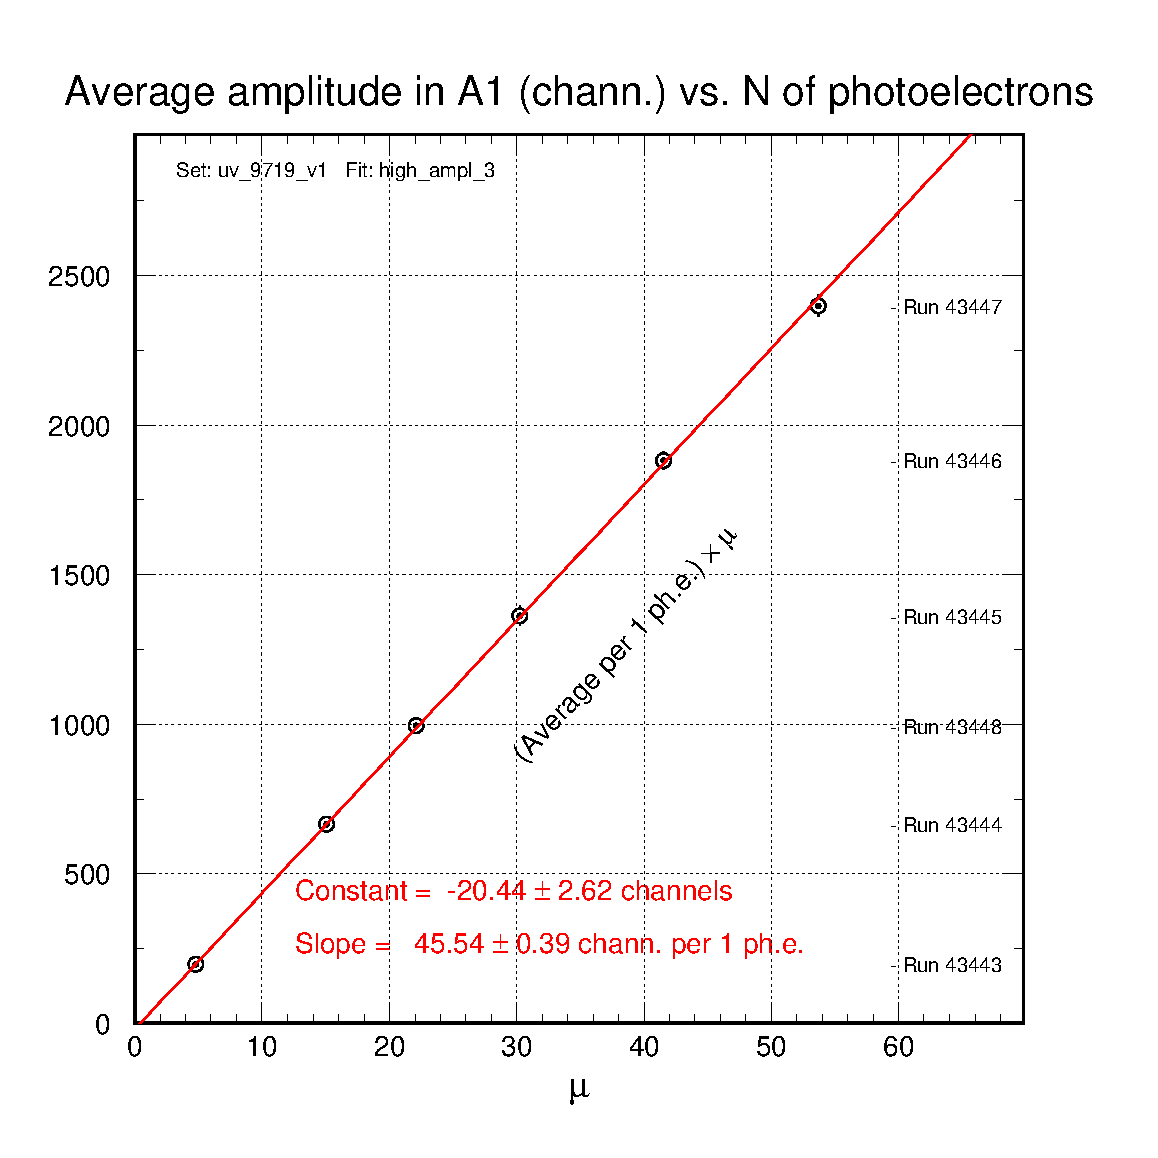
\includegraphics[height=8.0cm]{PMT-studies/uv_9719_v1_result.eps}
\vspace{0.5cm}
\caption{\small{Linear fits to the average ADC value vs. the average 
$N_{p.e.}$ of the Poisson distributions of the three UV glass-faced PMTs. 
The slopes are the ADC to $N_{p.e.}$ conversion factors.}}
\label{linear_uvglass}
\end{centering}
\end{figure}
%%%%%%%%%%%%%%%%%%%%%%%%%%%%%%%%%%%%%%%%%%%%%%%%%%%%%%%%%%%%%%%%%%%%%%%

%%%%%%%%%%%%%%%%%%%%%%%%%%%%%%%%%%%%%%%%%%%%%%%%%%%%%%%%%%%%%%%%%%%%%%%
\begin{figure}
\vspace{0.5cm}
\begin{centering}
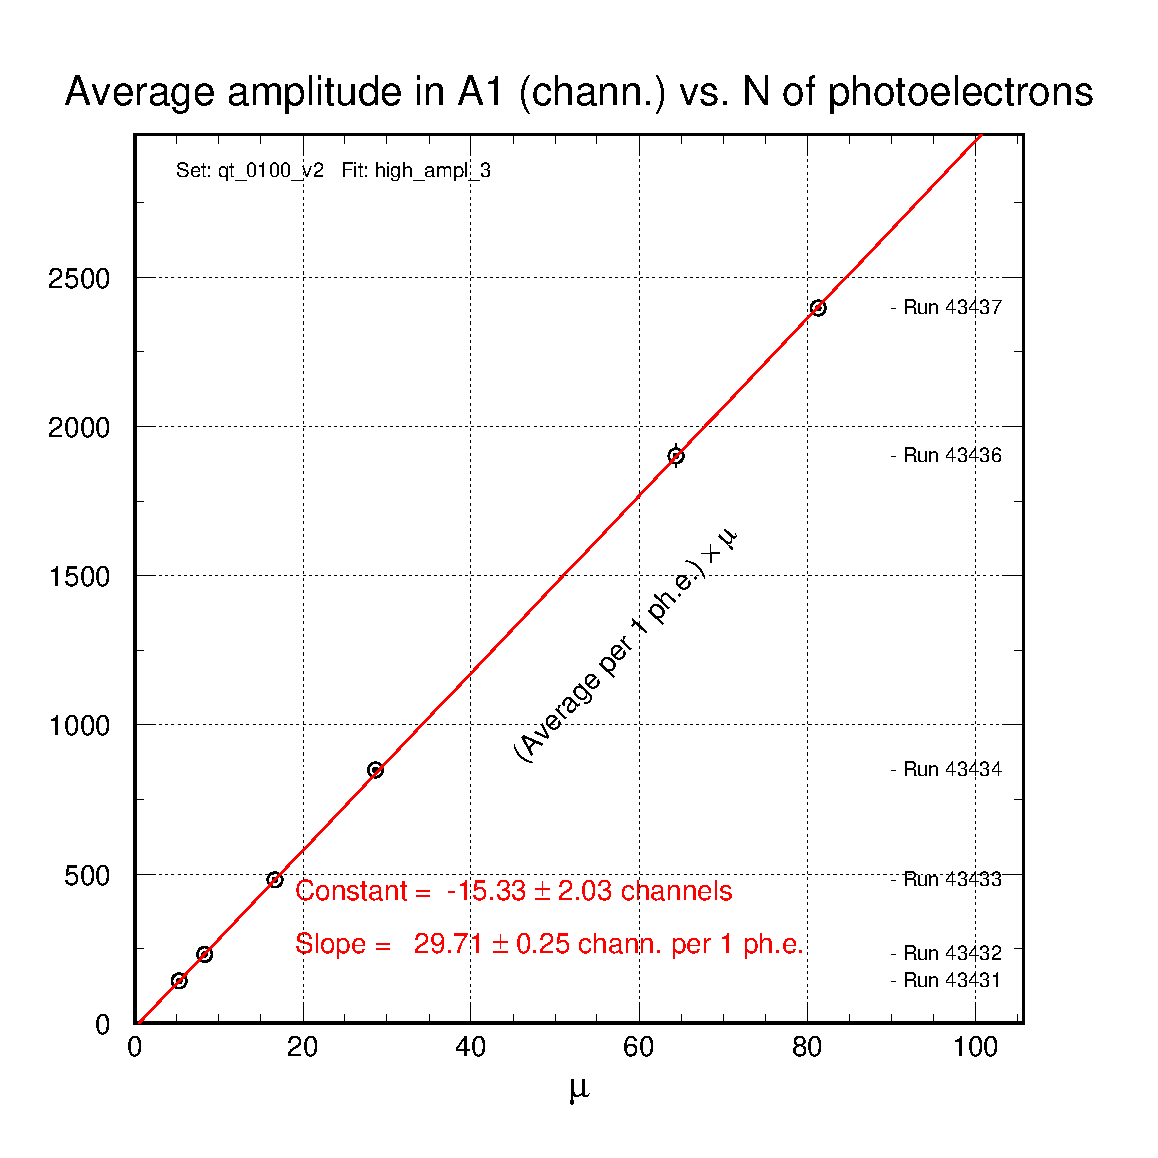
\includegraphics[height=8.5cm]{PMT-studies/qt_0100_v2_result.eps}
\end{centering}
\begin{centering}
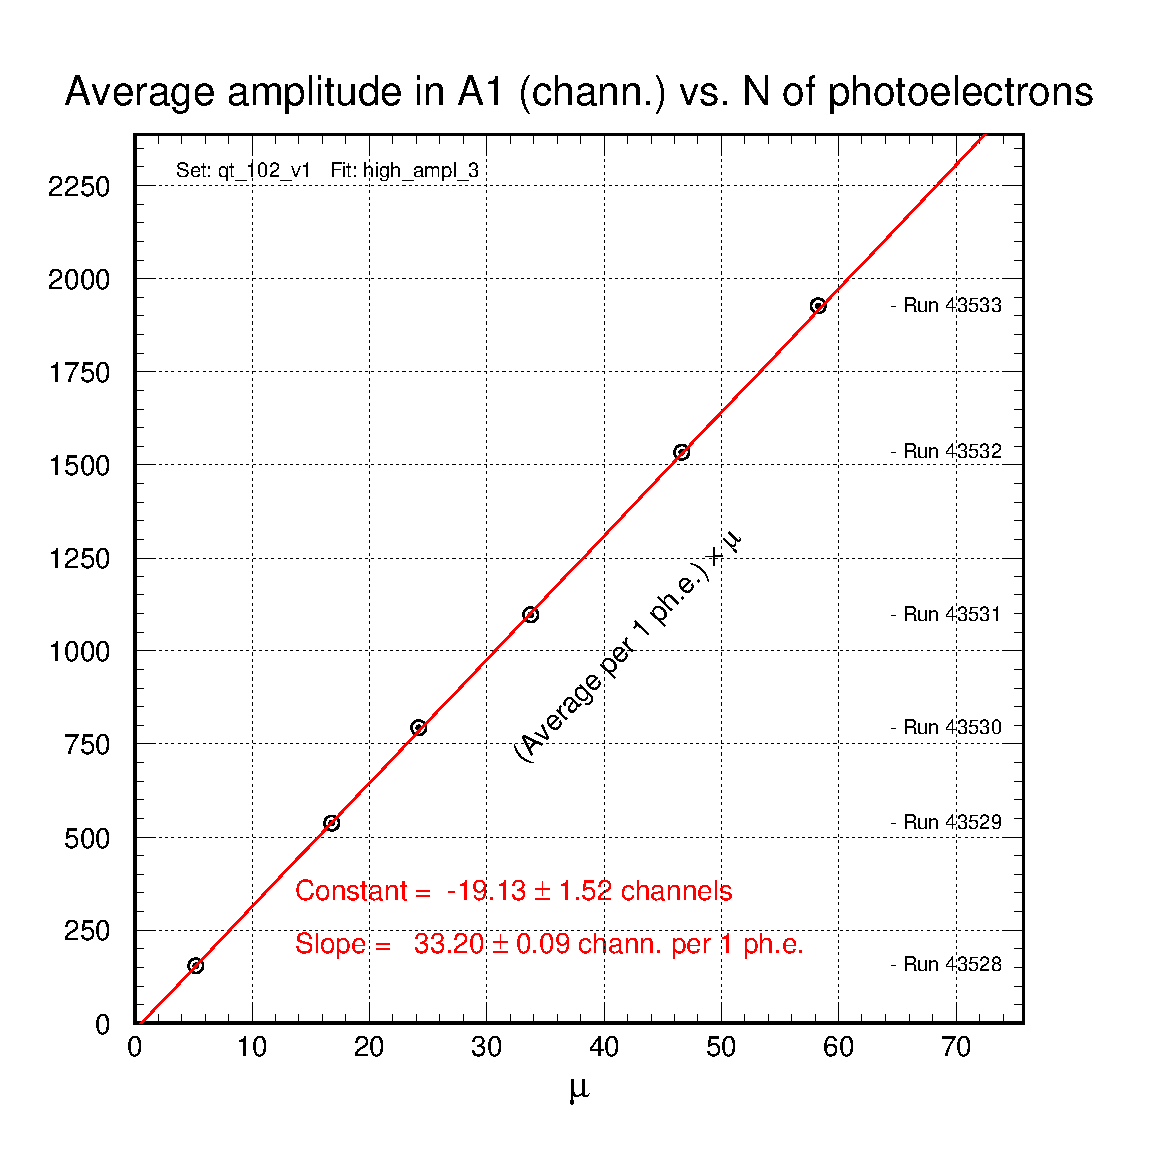
\includegraphics[height=8.0cm]{PMT-studies/qt_0102_v1_result.eps}
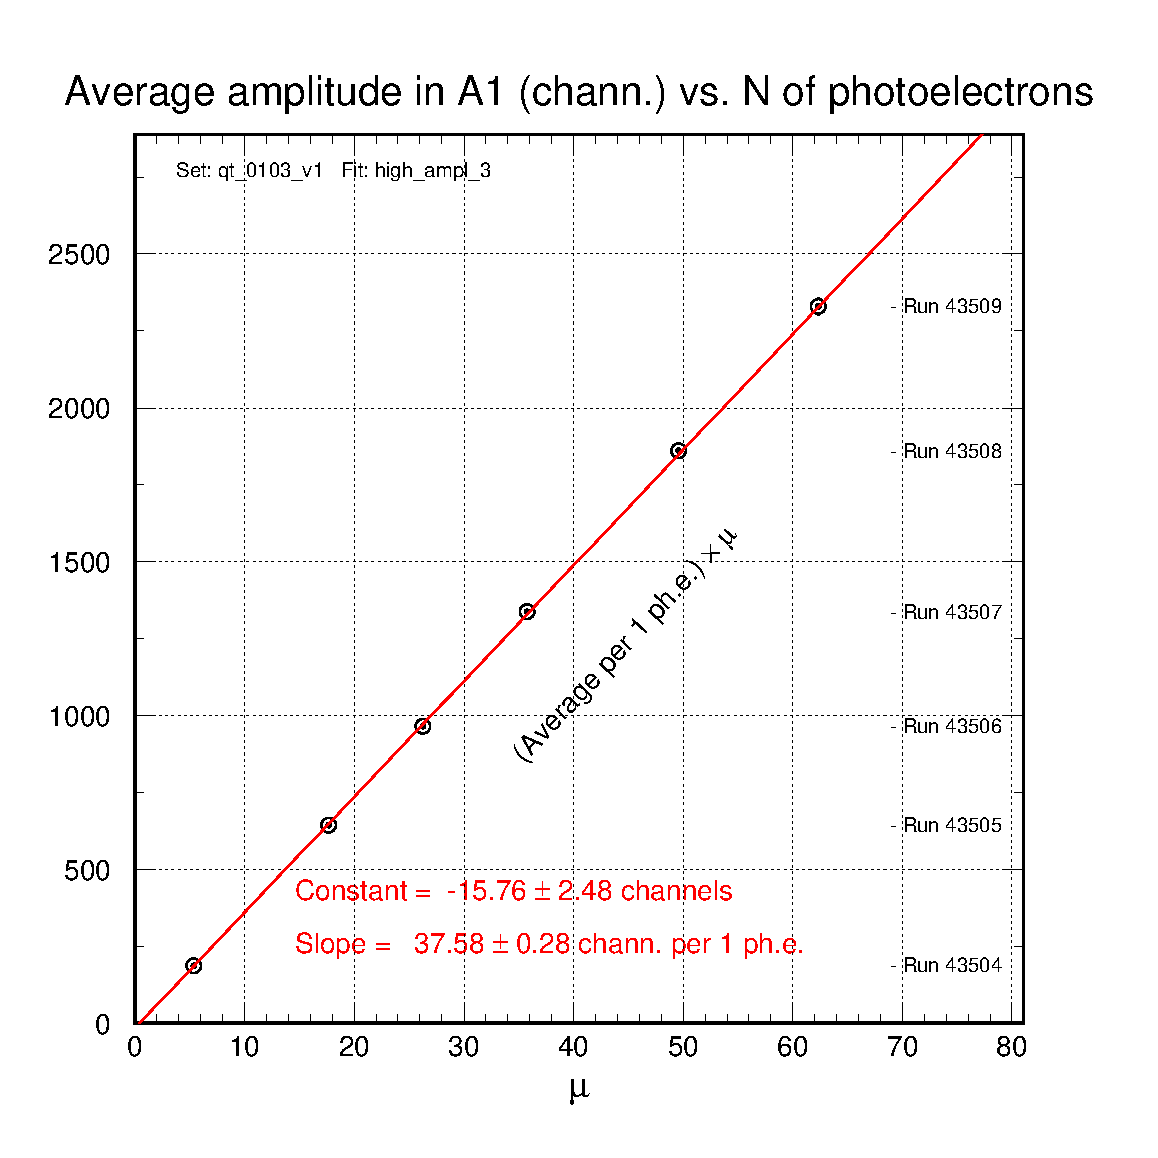
\includegraphics[height=8.0cm]{PMT-studies/qt_0103_v1_result.eps}
\vspace{0.5cm}
\caption{\small{Linear fits to the average ADC value vs. the average 
$N_{p.e.}$ of the Poisson distributions of the three quartz-faced PMTs.  
The slopes are the ADC to $N_{p.e.}$ conversion factors.}}
\label{linear_quartz}
\end{centering}
\end{figure}
%%%%%%%%%%%%%%%%%%%%%%%%%%%%%%%%%%%%%%%%%%%%%%%%%%%%%%%%%%%%%%%%%%%%%%%

To check that these conversion factors were correct, each PMT was tested
with the LED emitting only a single photon.  As seen in 
Fig.~\ref{numphe_check}, the conversion factors were applied to the ADC 
spectra and the mean number of photoelectrons for each distribution was 
approximately one, indicating that the conversion factors are correct. 

%%%%%%%%%%%%%%%%%%%%%%%%%%%%%%%%%%%%%%%%%%%%%%%%%%%%%%%%%%%%%%%%%%%%%%%
\begin{figure}
\hspace{0.5cm}
\begin{centering}
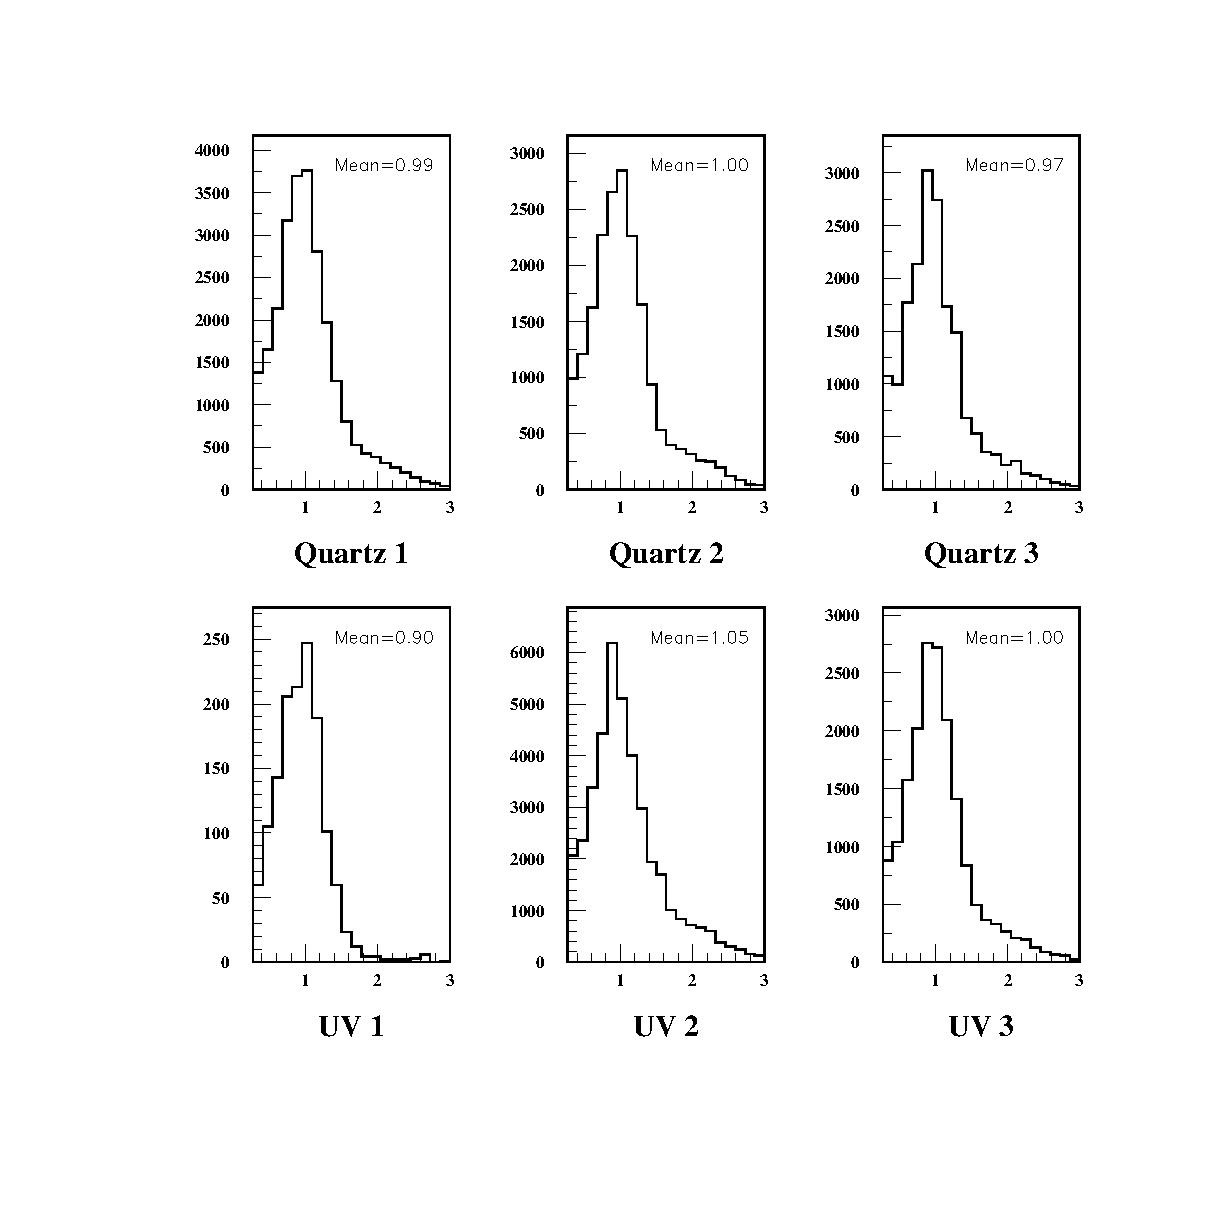
\includegraphics[height=10.5cm]{PMT-studies/al_phe.eps}
\vspace{0.5cm}
\caption{\small{$N_{p.e.}$ spectra for a single-photon LED source for 
the six test PMTs.  The means of each distribution are all near one, 
indicating that the ADC to $N_{p.e.}$ conversion factors are correct.}}
\label{numphe_check}
\end{centering}
\end{figure}
%%%%%%%%%%%%%%%%%%%%%%%%%%%%%%%%%%%%%%%%%%%%%%%%%%%%%%%%%%%%%%%%%%%%%%%

\subsubsection{{\v C}erenkov Light Test Results}

Using the ADC to $N_{p.e.}$ conversion factors, the three Photonis XP4508
quartz- and three Photonis XP4500 UV glass-faced PMTs were tested with 
the cosmic ray stand filled with air.  The results of the tests, with each
measured for about a week, are shown in Fig.~\ref{numphe_all}, which
highlights the $N_{p.e.}$ spectra from collecting the {\v C}erenkov
radiation.  Fig.~\ref{avg_numphe} illustrates the average $N_{p.e.}$ for 
each PMT-face type, yielding an increase of $45 \pm 4$\% in the number of 
detected {\v C}erenkov photoelectrons in quartz-faced PMTs over UV 
glass-faced PMTs.  This result is larger than the predicted increase of 20\% 
found in eq.(\ref{eq:light_ratio}).  This difference is most likely due to 
an error in the rough quantum efficiency estimate that the manufacturer 
supplied.  Fig.~\ref{ref_pmt} shows a fit to the average number of 
photoelectrons collected by the quartz reference PMT throughout the two 
months of testing.  In five tests, the maximum deviation from the average of 
58 photoelectrons was 4.1\%, which may be considered as an estimate of the 
systematic uncertainty of the experiment. 

%%%%%%%%%%%%%%%%%%%%%%%%%%%%%%%%%%%%%%%%%%%%%%%%%%%%%%%%%%%%%%%%%%%%%%%
\begin{figure}
\hspace{0.5cm}
\begin{centering}
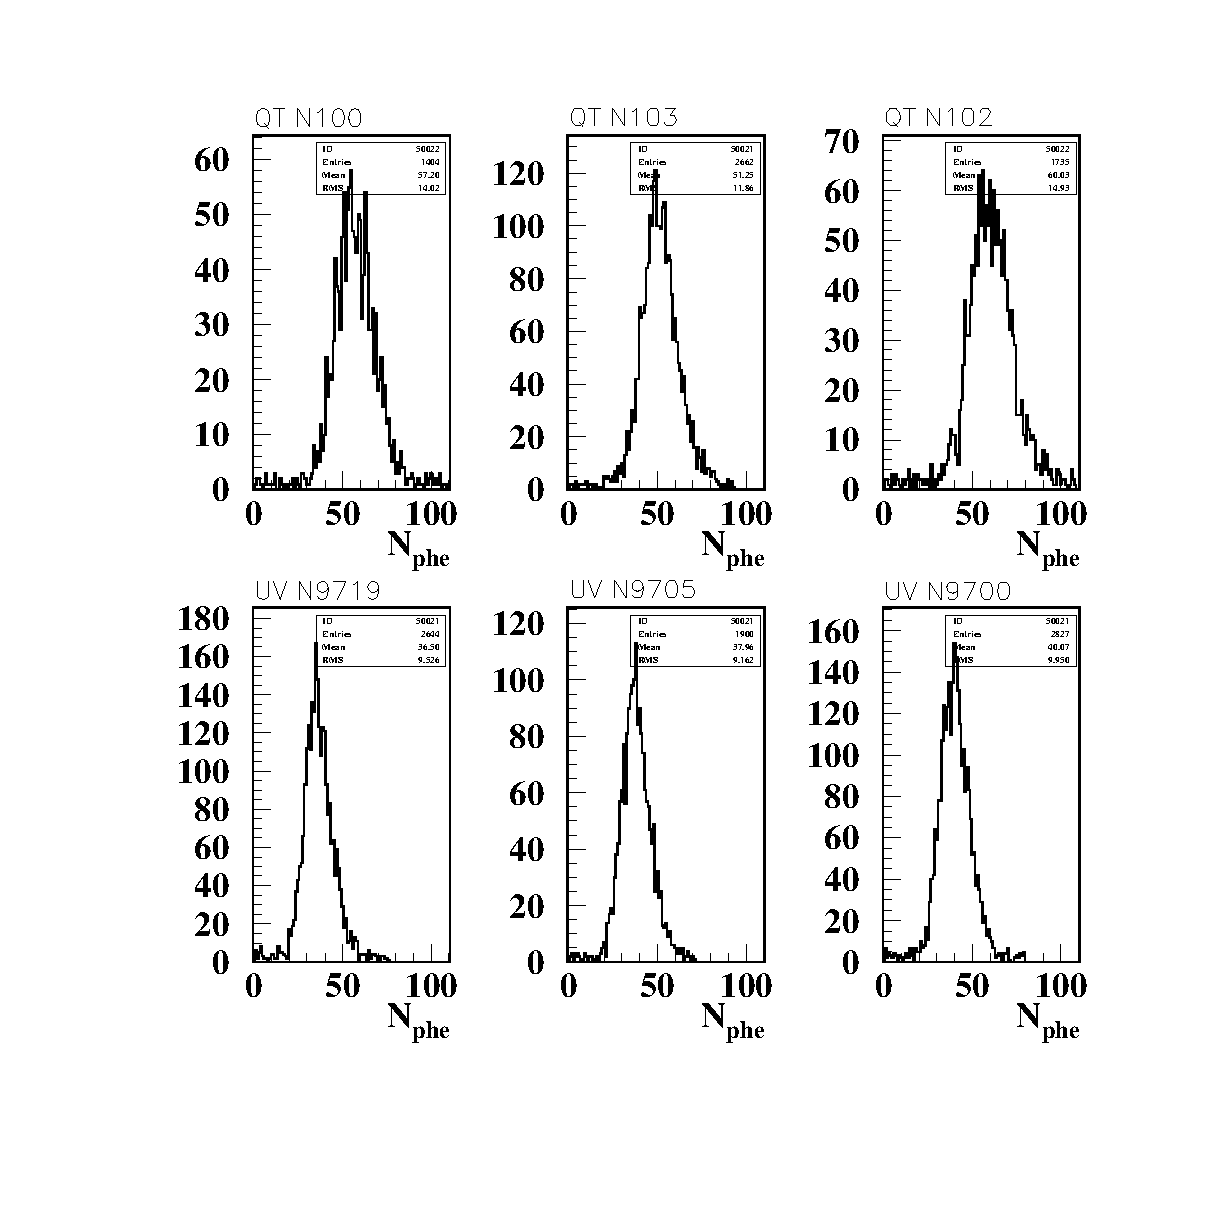
\includegraphics[height=10.5cm]{PMT-studies/all_phe_spectra.eps}
\vspace{0.5cm}
\caption{\small{$N_{p.e.}$ spectra from collecting {\v C}erenkov light in 
the cosmic ray stand for the three UV glass- and three quartz-faced PMTs.}}
\label{numphe_all}
\end{centering}
\end{figure}
%%%%%%%%%%%%%%%%%%%%%%%%%%%%%%%%%%%%%%%%%%%%%%%%%%%%%%%%%%%%%%%%%%%%%%%

%%%%%%%%%%%%%%%%%%%%%%%%%%%%%%%%%%%%%%%%%%%%%%%%%%%%%%%%%%%%%%%%%%%%%%%
\begin{figure}
\hspace{0.5cm}
\begin{centering}
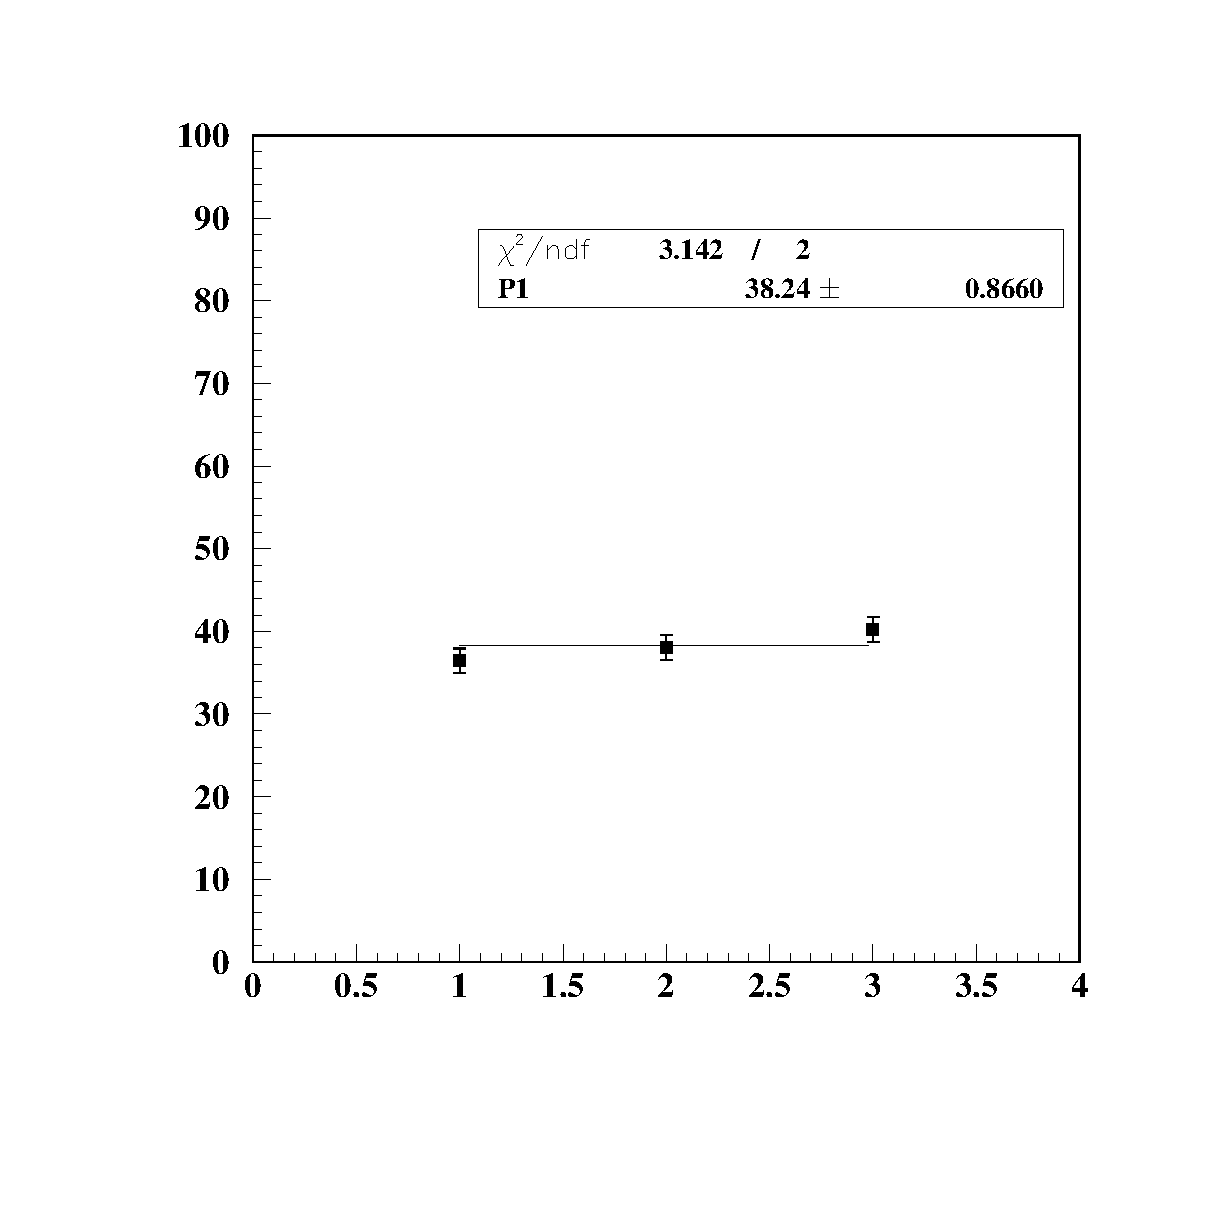
\includegraphics[height=7.5cm]{PMT-studies/uv.eps}
\includegraphics[height=7.5cm]{PMT-studies/qt.eps}
\vspace{0.5cm}
\caption{\small{Fits to find the average $N_{p.e.}$ for UV glass- and 
quartz-faced PMTs.}}
\label{avg_numphe}
\end{centering}
\end{figure}
%%%%%%%%%%%%%%%%%%%%%%%%%%%%%%%%%%%%%%%%%%%%%%%%%%%%%%%%%%%%%%%%%%%%%%%

%%%%%%%%%%%%%%%%%%%%%%%%%%%%%%%%%%%%%%%%%%%%%%%%%%%%%%%%%%%%%%%%%%%%%%%
\begin{figure}
\hspace{0.5cm}
\begin{centering}
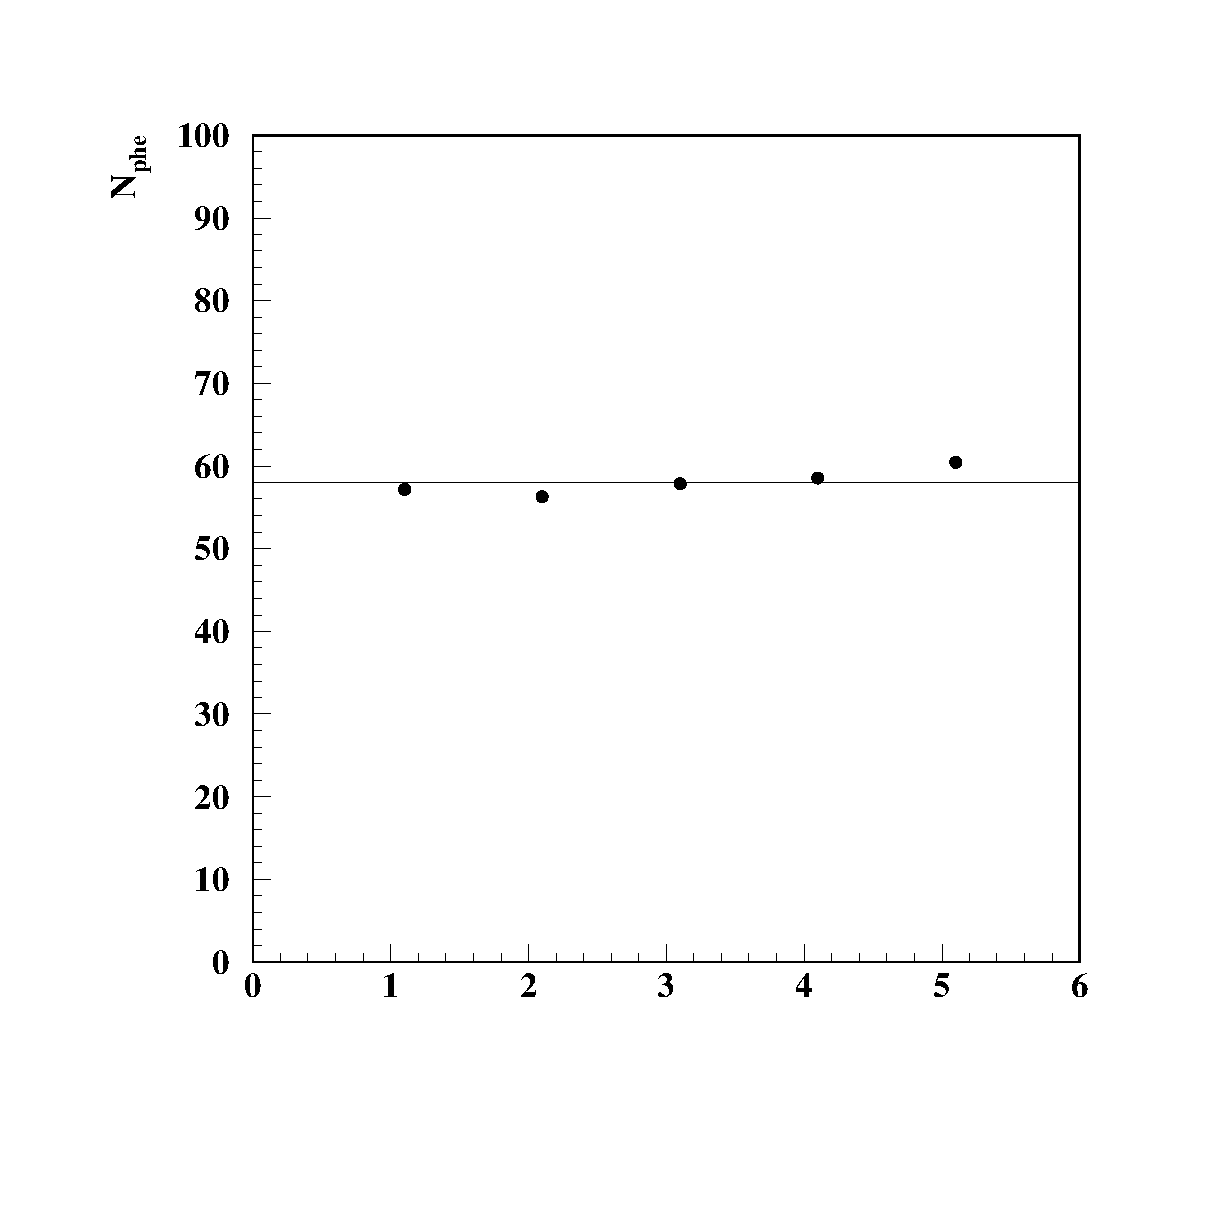
\includegraphics[height=9.5cm]{PMT-studies/stab.eps}
\vspace{0.5cm}
\caption{\small{The number of photoelectrons collected by the reference 
PMT during testing.  The maximum deviation of 4.1\% is a reflection of 
the systematic uncertainty of the experiment.}}
\label{ref_pmt}
\end{centering}
 \end{figure}
%%%%%%%%%%%%%%%%%%%%%%%%%%%%%%%%%%%%%%%%%%%%%%%%%%%%%%%%%%%%%%%%%%%%%%%

%%%%%%%%%%%%%%%%%%%%%%%%%%%%%%%%%%%%%%%%%%%%%%%%%%%%%%%%%%%%%%%%%%%%%%%
\begin{figure}
\hspace{0.5cm}
\begin{centering}
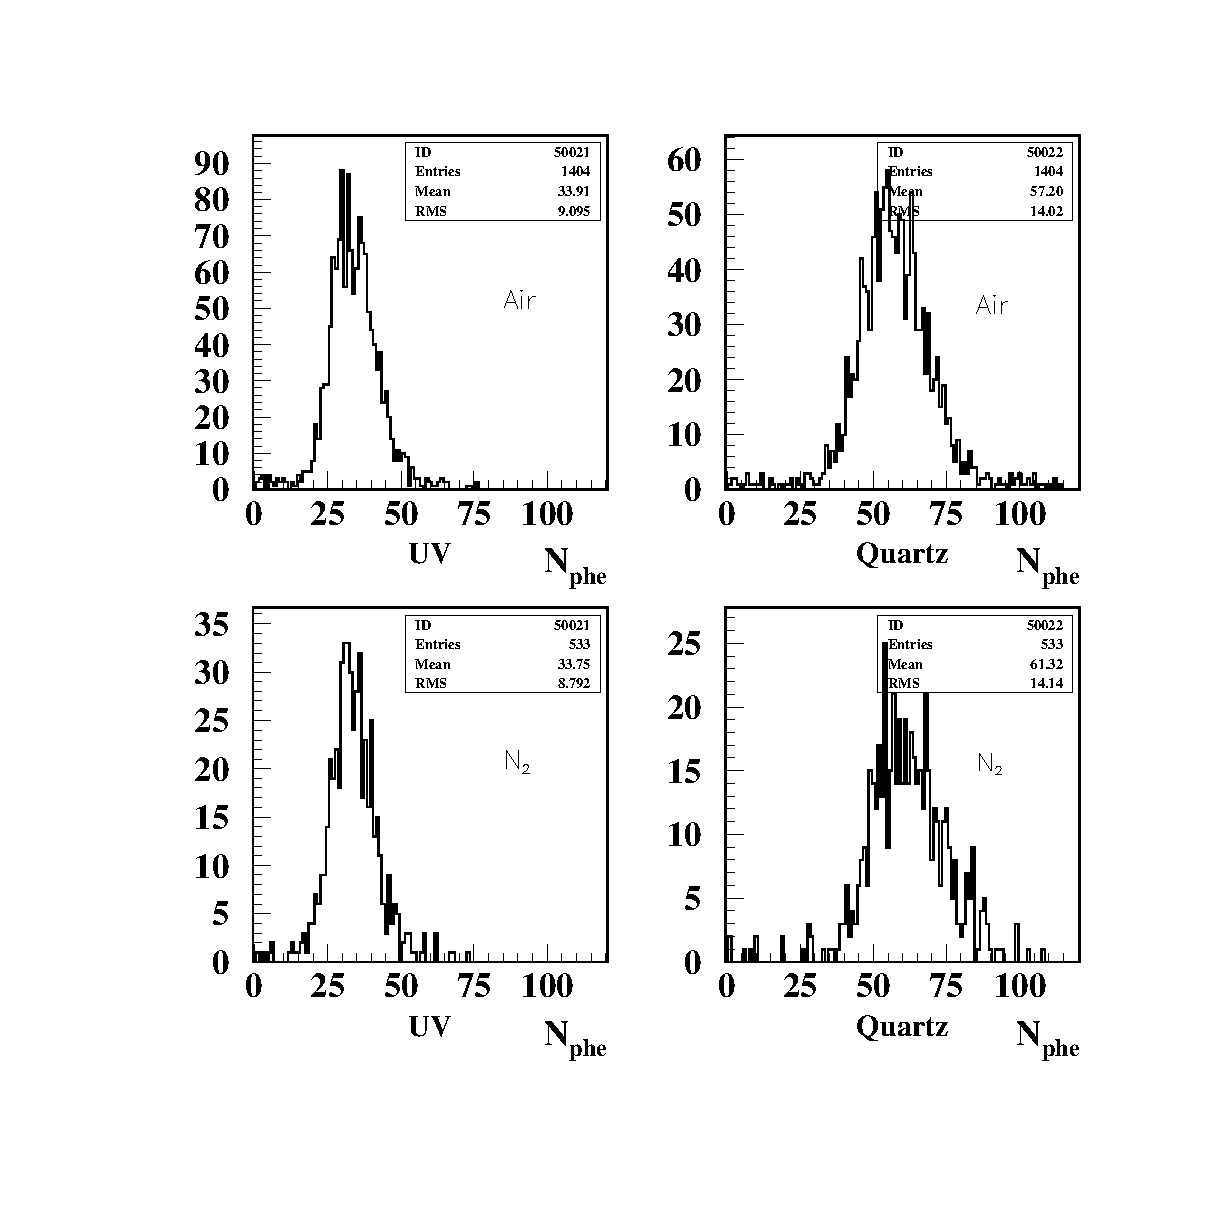
\includegraphics[height=9.5cm]{PMT-studies/gas_spectra.eps}
\vspace{0.5cm}
\caption{\small{$N_{p.e.}$ spectra for UV-glass and quartz-faced PMTs in 
a nitrogen gas environment.}}
\label{ntogas}
\end{centering}
\end{figure}
%%%%%%%%%%%%%%%%%%%%%%%%%%%%%%%%%%%%%%%%%%%%%%%%%%%%%%%%%%%%%%%%%%%%%%%

%%%%%%%%%%%%%%%%%%%%%%%%%%%%%%%%%%%%%%%%%%%%%%%%%%%%%%%%%%%%%%%%%%%%%%%
\begin{figure}
\hspace{0.5cm}
\begin{centering}
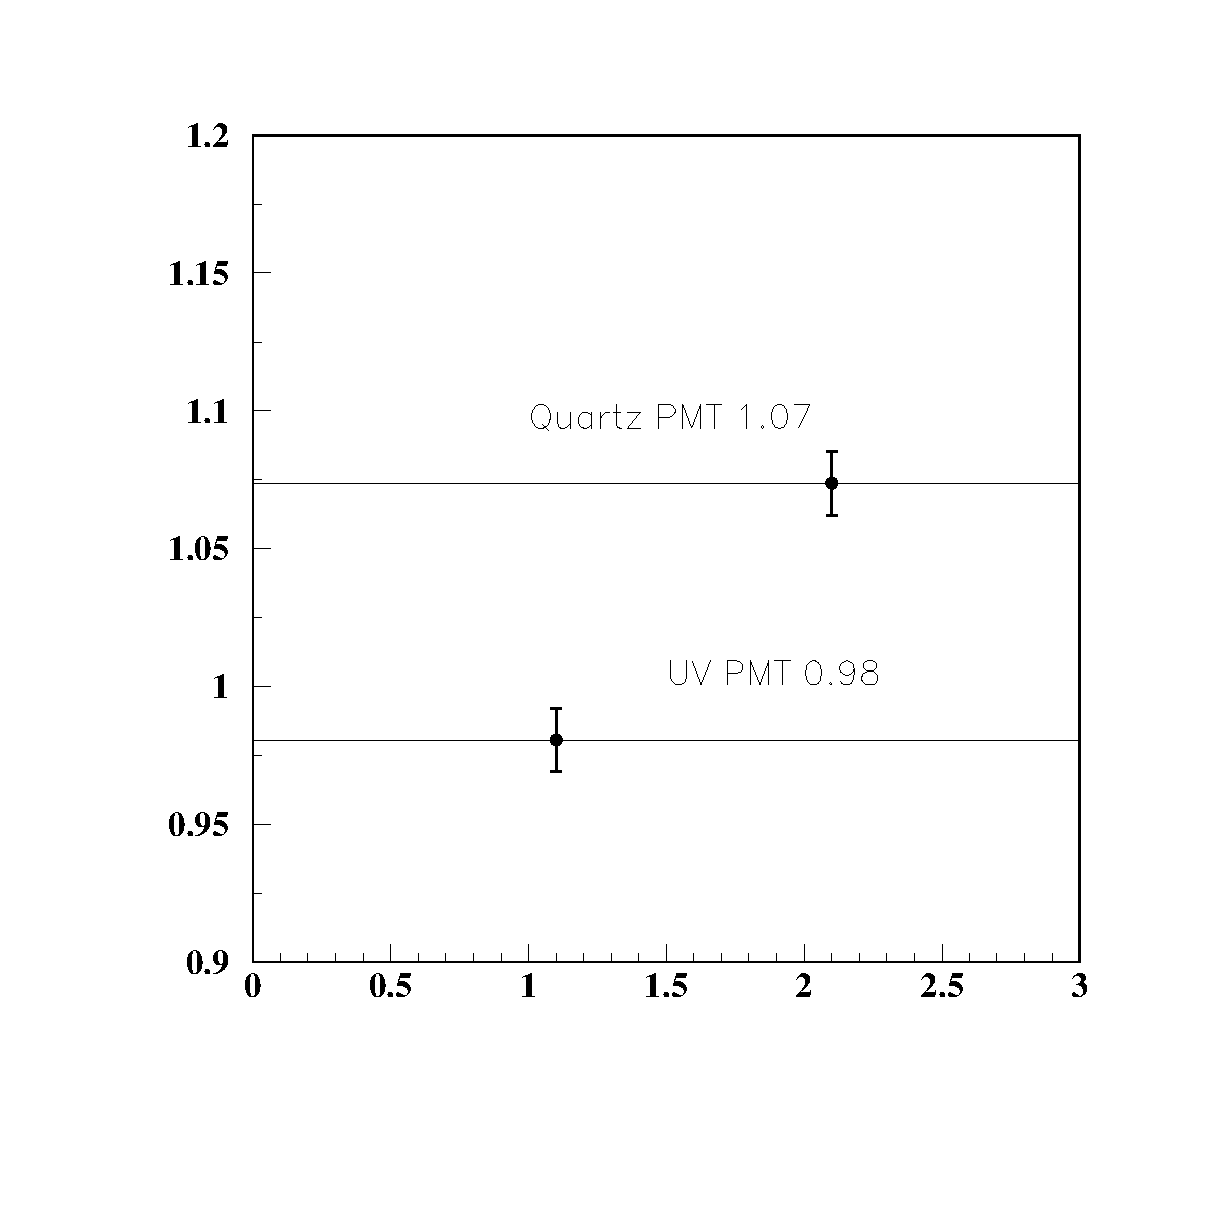
\includegraphics[height=9.5cm]{PMT-studies/gas.eps}
\vspace{0.5cm}
\caption{\small{Ratio of light collection in nitrogen gas to the air 
environment for UV-glass and quartz`faced PMTs.}}
\label{gas}
\end{centering}
\end{figure}
%%%%%%%%%%%%%%%%%%%%%%%%%%%%%%%%%%%%%%%%%%%%%%%%%%%%%%%%%%%%%%%%%%%%%%%

One quartz- and one UV glass-faced PMT were tested in the cosmic ray
stand with the chamber filled with nitrogen gas.  Fig.~\ref{ntogas}
illustrates the $N_{p.e.}$ spectra for these tests, yielding an average
photoelectron detection increase of 82\%.  This is much larger than
the predicted increase of 25\% from Section~\ref{sec:Cerenkov-Light-Detection}.
As mentioned previously, the rough quantum efficiency distributions
supplied by Photonis are likely incorrect.  Additionally, only one PMT 
of each type was tested; thus this difference may be inflated by the 
inconsistent response between PMTs of the same model.  So, this estimate 
based on a single measurement is very crude.  The amount of light collected 
by the quartz-faced PMT in a nitrogen gas environment was 7\% more than in 
air, similar to the predicted increase of 4.5\% from
Section~\ref{sec:Cerenkov-Light-Detection}.  The amount of light collected 
by the UV glass-faced PMT actually decreased by 2\% in nitrogen gas, as 
opposed to the negligible difference that was predicted (see Fig.~\ref{gas}). 

In summary, using a cosmic ray test stand, the Photonis XP4508 quartz-faced 
PMTs were found to collect 45\% more {\v C}erenkov radiated photoelectrons
in air than the Photonis XP4500 UV glass-faced PMTs.  In a nitrogen gas 
environment, the {\v C}erenkov light collection of the quartz-faced
PMTs improved by an additional 7\%, so the total gain is estimated  
to be 55\% ($1.45\times1.07$=1.55). 
